%%%%%%%%%%%%%%%%%%%%%%%%%%%%%%%%%%%%%%%%%%%%%%%%%%%%%%%%%%%%%%%%%%%%
%% I, the copyright holder of this work, release this work into the
%% public domain. This applies worldwide. In some countries this may
%% not be legally possible; if so: I grant anyone the right to use
%% this work for any purpose, without any conditions, unless such
%% conditions are required by law.
%%%%%%%%%%%%%%%%%%%%%%%%%%%%%%%%%%%%%%%%%%%%%%%%%%%%%%%%%%%%%%%%%%%%

\documentclass[
  digital, %% The `digital` option enables the default options for the
           %% digital version of a document. Replace with `printed`
           %% to enable the default options for the printed version
           %% of a document.
%%  color,   %% Uncomment these lines (by removing the %% at the
%%           %% beginning) to use color in the printed version of your
%%           %% document
  oneside, %% The `oneside` option enables one-sided typesetting,
           %% which is preferred if you are only going to submit a
           %% digital version of your thesis. Replace with `twoside`
           %% for double-sided typesetting if you are planning to
           %% also print your thesis. For double-sided typesetting,
           %% use at least 120 g/m² paper to prevent show-through.
  lof,     %% The `lof` option prints the List of Figures. Replace
           %% with `nolof` to hide the List of Figures.
  nolot,     %% The `lot` option prints the List of Tables. Replace
           %% with `nolot` to hide the List of Tables.
]{fithesis4}
%% The following section sets up the locales used in the thesis.
\usepackage[resetfonts]{cmap} %% We need to load the T2A font encoding
\usepackage{latex-javaScript/jslistings}
\usepackage[T1,T2A]{fontenc}  %% to use the Cyrillic fonts with Russian texts.
\usepackage[
  main=english, %% By using `czech` or `slovak` as the main locale
                %% instead of `english`, you can typeset the thesis
                %% in either Czech or Slovak, respectively.
  english, german, russian, czech, slovak %% The additional keys allow
]{babel}        %% foreign texts to be typeset as follows:
%%
%%   \begin{otherlanguage}{german}  ... \end{otherlanguage}
%%   \begin{otherlanguage}{russian} ... \end{otherlanguage}
%%   \begin{otherlanguage}{czech}   ... \end{otherlanguage}
%%   \begin{otherlanguage}{slovak}  ... \end{otherlanguage}
%%
%% For non-Latin scripts, it may be necessary to load additional
%% fonts:
\usepackage{paratype}
\usepackage{my-alias}
\def\textrussian#1{{\usefont{T2A}{PTSerif-TLF}{m}{rm}#1}}
%%
%% The following section sets up the metadata of the thesis.
\thesissetup{
    date        = \the\year/\the\month/\the\day,
    university  = mu,
    faculty     = fi,
    type        = bc,
    department  = Department of Computer Science,
    author      = Adam Hlaváček,
    gender      = m,
    advisor     = {RNDr. Vladimír Štill, Ph.D.},
    title       = {Revitalization and Modernization of Web Application of the Online Seminar of Informatics},
    TeXtitle    = {Revitalization and Modernization of Web Application of the Online Seminar of Informatics},
    keywords    = {KSI, web application, frontend, TypeScript, Python, Angular},
    TeXkeywords = {KSI, web application, frontend, TypeScript, Python, Angular},
    abstract    = {%
      This thesis aims to solve the degrading state of the web application of the Online Seminar of Informatics (KSI). The current web application is built upon an unsupported web framework, which cannot be easily updated to its supported version. To resolve this issue, this thesis creates a new implementation of the said web application, which will use a technology that is expected to be maintainable in the long term. First, it discusses which technology is best suited for a given use case and then presents the solution, together with changes made to the KSI backend and a new KSI frontend. As a result, the new web application is shown with two active deployments. One of which is used as a production environment for a new online seminar, which is possible due to the high focus on easy modularity throughout the development process.
    },
    thanks      = {%
       I want to thank my advisor, RNDr. Vladimír Štill, Ph.D., for his invaluable insights and advice throughout this thesis. Likewise, I would like to thank the entire KSI organizers team for frequent feedback and words of encouragement during the development process. Finally, I would like to express my gratitude to my girlfriend and family for their everlasting support.
    },
    bib         = thesis.bib,
    %% Remove the following line to use the JVS 2018 faculty logo.
    facultyLogo = fithesis-fi,
}
\usepackage{makeidx}      %% The `makeidx` package contains
\makeindex                %% helper commands for index typesetting.
\usepackage[acronym]{glossaries}          %% The `glossaries` package
\renewcommand*\glspostdescription{\hfill} %% contains helper commands
\loadglsentries{abbreviations.tex}  %% for typesetting glossaries
\makenoidxglossaries                      %% and lists of abbreviations.
%% These additional packages are used within the document:
\usepackage{paralist} %% Compact list environments
\usepackage{amsmath}  %% Mathematics
\usepackage{amsthm}
\usepackage{amsfonts}
\usepackage{url}      %% Hyperlinks
\usepackage{markdown} %% Lightweight markup
\usepackage{listings} %% Source code highlighting
\lstset{
  basicstyle      = \ttfamily,
  identifierstyle = \color{black},
  keywordstyle    = \color{blue},
  keywordstyle    = {[2]\color{cyan}},
  keywordstyle    = {[3]\color{olive}},
  stringstyle     = \color{teal},
  commentstyle    = \itshape\color{magenta},
  breaklines      = true,
}
\usepackage{floatrow} %% Putting captions above tables
\floatsetup[table]{capposition=top}
\usepackage[babel]{csquotes} %% Context-sensitive quotation marks
\begin{document}
%% Uncomment the following lines (by removing the %% at the beginning)
%% and to print out List of Abbreviations and/or Glossary in your
%% document. Titles for these tables can be changed by replacing the
%% titles `Abbreviations` and `Glossary`, respectively.
\clearpage
\printnoidxglossary[title={Abbreviations}, type=\acronymtype]
\printnoidxglossary[title={Glossary}]

%% The \chapter* command can be used to produce unnumbered chapters:
\chapter*{Introduction}
%% Unlike \chapter, \chapter* does not update the headings and does not
%% enter the chapter to the table of contents. I we want correct
%% headings and a table of contents entry, we must add them manually:

\mdstart

The Online Seminar of Informatics (KSI for short) is an annual online competition and also one of the activities of the Faculty of Informatics targeted at high school students. The central part of \acrshort{KSI} takes place from September to April in four thematic waves. Each wave consists of at least a dozen tasks in which the participants can learn and then apply various informatics principles. Participants who earn a minimum of 60\% points for completing given tasks awarded throughout all four waves are suitable to be accepted to the Faculty of Informatics without taking entrance exams. Every year \acrshort{KSI} has more than five hundred participants who solve the tasks on its current website located at \href{https://ksi.fi.muni.cz}{ksi.fi.muni.cz}.

The current website is created with an outdated framework with linked security implications, and only a fraction of the current organizers have the needed understanding of code. Because of this, the main goal of this thesis is to create a new web application for \acrshort{KSI}, with the primary focus on easy and effective maintenance in terms of long term support.

The secondary goals of this thesis are for the new web application to make the website usable on mobile devices, present older tasks incompatible with the current website and improve the overall user experience of the web page.

As a part of this thesis, related modifications are also made to the server part of the \acrshort{KSI} infrastructure.

The first chapter describes what requirements are laid upon the \acrshort{KSI} web application. The second chapter depicts the current \acrshort{KSI} infrastructure, both frontend and backend. The third chapter discusses possible approaches to the development of new web application. Chapters 4 and 5 present the newly created projects for manipulation with the backend and the new web application, respectively. The final web application, which is the primary goal of this thesis, is already publicly deployed both for \fnurl{KSI}{https://ksi.fi.muni.cz/novy-web/} and a new online seminar \fnurl{Jump-start the \acrshort{FI}}{https://naskoc.fi.muni.cz/}.

\end{markdown*}

\markright{\textsc{Introduction}}
\addcontentsline{toc}{chapter}{Introduction}

\mdchap{Components of the \acrshort{KSI} web application}

Given that a web frontend for \acrshort{KSI} already exists and this thesis aims to be a revitalization of the \acrshort{KSI} frontend, it is expected that the new web frontend will implement the same features as can be found in the current one. These features are discussed in separate sub-chapters.

#### Learning task

The \acrshort{KSI} participants will spend most of their time on pages containing tasks. Every task has an assignment text, in which the subject of a given task is first explained and then examined in so-called modules. Modules can take the following forms:

- single choice question
- multiple choice question
- text input question (the participant must write the correct answer)
- programming task (the participant has to write a code that passes hidden tests)
- sorting task (the participant is tasked with rearranging code blocks into correct order)
- uploading a file (primarily used for tasks that are manually reviewed and evaluated)

Every module has a certain number of points awarded to the participant based on user's answers, and a single task can have multiple modules. Moreover, every task has its discussion thread in which participants can submit their questions. An original solution to the task is made available to the participant after the successful submission of the task.

All tasks are grouped into thematic units -- waves -- which gradually explain a single subject to the participant. Because a task often requires knowledge of content from other tasks, the tasks can be ordered so that, to unlock one task, the participant has to solve all previous tasks. This prerequisite is best represented as a directed acyclic graph, which must be visible to the participants for easier orientation.

#### Discussion

Unlike the discussion attached to every task, a general discussion with custom-named threads is required because some participants' questions are not related to a single task. Any registered user can create a new thread in this general discussion.

#### Results

The participants are sorted based on their earned number of points on a results page. The \acrshort{KSI} differentiates participants from high school and others. If the participant gains at least 60 \% of all available points from all tasks, the user is awarded the title of a successful participant. Such participant needs to have a different colour in the results table. Furthermore, every user can be granted an achievement trophy for completing a particular assignment. Every such trophy needs a page with its description and icon.

#### General features

Because \acrshort{KSI} is an annual competition, the frontend needs to present an option for selecting which year should be displayed to the user. The web application should also support logging in for already registered users and registering new users. Every registered user should have a public profile with part of the information visible only after logging in (for example, the user's email should not be visible in the public version of user's profile).

Pages with information about the online seminar itself and about news in the current year are also to be included.

\end{markdown*}

\mdchap{KSI Infrastrucute}

KSI's organizers manage two virtual servers hosted on faculty's Open Nebula platform, both running Debian OS. One of these servers is for production, the second is for testing. Both share the same format -- an Apache web server, which server the frontend and reverse proxies the backend.
The production server is called `kleobis` and the development `kyzikos` and I will refer to them troughout this thesis as such.

Kleobis has assigned two domains -- \href{https://ksi.fi.muni.cz}{ksi.fi.muni.cz} for access to the frontend and \href{https://rest.ksi.fi.muni.cz}{rest.ksi.fi.muni.cz} for calling backend endpoints.

Kyzikos has no public access, because it is meant as a development server on which the organizers can test their possibly breaking modification without interfering with the production instance.

The frontend~[@ksi-web-frontend] can be automatically deployed from its repository by building it using GitHub Actions and then copying the built web application on the desired server by calling an automated script on one of the organizers faculty accounts.

The backend~[@ksi-web-backend] has no means for automatic deployment and updating. The process has to be performed manualy, by logging into target server, pulling from the source code repository and performing a manual restart. This is a desired workflow, because updates to the backend server are infrequent and a manual check of functionality after an update increases certanity that the server will work as desired even after the update.

## Frontend

### Maintenance of the current frontend

The current web frontend of the Online Seminar of Informatics (KSI for short) was written using the first version of the Ember.js framework. The last minor version of the first version of the Ember.js framework was released on the 12th of June 2015~[@ember-1]. The frontend stayed principally the same throughout the years because the first Ember.js version cannot be upgraded to a more recent and supported version with ease. Following the fact that Ember v1 was released in 2015, present seminar organizers face a few severe issues -- the foremost being security implications of using old and deprecated software and the second being the lack of volunteers with enough knowledge of this technology. In its current state, the frontend is singlehandedly managed by Ondřej Borýsek~[@ksi-web-frontend].

Since the support of the used framework ended, the organizers have been aware of these issues. They have tried to migrate the used version to a current stable version of Ember, most notably inside a private project called web-frontend-ember3~[@ksi-web-frontend-ember3], but these attempts were not successful. The leading explanation for the prevalence of the current frontend is that all organizers are volunteers. With only a limited amount of time available, the organizers decided to work on more imminent duties. However, this task has gained a significant priority as Ondřej Borýsek will finish his studies shortly. Consequently, none of the team members will be capable of resolving issues or implementing new features.

### Possible solutions

When deciding how to approach the development of the new version of the \acrshort{KSI} frontend, I was faced with three viable alternatives. The first option was to adapt the web of any similarly focused seminar, which was deemed inappropriate because the \acrshort{KSI} has developed its backend with unique features not easily adaptable from other projects. The second possibility was to continue with a previous attempt to upgrade the frontend to the newer version of the Ember framework. This option was also discarded as there is a risk that the project would be eventually hard to manage, similarly to the current state. As per the Stack Overflow 2020 developer survey~[@stackoverflow-survey], the Ember framework is no longer used regularly and thus unsuitable for a long-lasting project.

The last option was to develop a new project from scratch using one of the most used web frameworks. Besides jQuery, which is not a full-featured web framework, the most used ones are React.js and Angular~[@stackoverflow-survey].

React.js~[@react-github], developed by Meta, is the most popular~[@stackoverflow-survey] full-featured web framework. It is focused on the fast development of responsive web applications while heavily depending on modularity and supporting it via external libraries. This modularity allows the developer to tailor the project's library set precisely for the project's needs. Since component logic in React.js is written in JavaScript instead of templates, it is easy to pass rich data through the applications and keep the state out of the DOM~[@reactjs]. An added benefit of React.js is that it is taught on the Faculty of Informatics at Masaryk University in a course called Modern Markup Languages and Their Applications, which is compulsory for both
Programming and Development~[@fi-pva] program and some specializations of Informatics~[@fi-inf]. Nevertheless, most of the current members of the organizer teams have no experience with web development whatsoever; hence choosing React.js is not fundamental.

Angular~[@angular], developed by Google, on the other hand, includes most of the frequently used features~[@angular-features] like routing, \acrshort{HTTP} client, forms manipulation, and internalization. Therefore Angular allows the developers to get familiar with a new project more rapidly without needing to learn about new third-party libraries used within a given project.

Because the team of seminar organizers changes quite frequently, it is crucial to minimize the entrance barrier for new developers to be capable of modifying the frontend. A lower entrance barrier can be achieved by using a well-established technology with minimal supplementary knowledge. Concerning precisely that argumentation, Angular was chosen as more fitting and is utilized throughout this thesis.

## Backend

The backend server~[@ksi-web-backend] is written as a Python 3 project and acts mainly as a middle-ware between the user and the database. A heavily utilized part of the backend is its capability to execute untrusted code sandboxed, which is crucial for \acrshort{KSI}. The backend is used for manipulating with a git repository containing data of tasks for the participants to solve (assignment, solution and optional additional assets).

### Code sandboxing

To sandbox untrusted code, mainly originating from participant's task evaluations, KSI uses the `isolate`~[@isolate] project. This project was developed for the needs of programming contests, so it perfectly fits \acrshort{KSI}'s needs. It uses so-called boxes, in which an executed command has only a limited but fully defined set of capabilities. This can mitigate the risk of overloading the host's system by a program stuck in a neverending loop, using the host's network as a point of entry for an attacker or even gaining direct access to the host's system.

### Python web framework

The \acrshort{KSI} backend utilizes the Falcon~[@falcon] framework for handling all \acrshort{HTTP} \acrshort{API} calls, which companies like PayPal and LinkedIn~[@falcon-usage] use. This framework is optimized for creating RESTful~[@rest] API and is better suitable for a larger volume of incoming requests. Every endpoint is defined as a class that has an implemented method for every supported \acrshort{HTTP} method. This Python class method is given two parameters -- `request` and `response`. This simplicity of the framework design allows for easy and quick implementation of new endpoints and a steep learning curve for new project maintainers.

\end{markdown*}

\mdchap{Selecting framework for a new web application}

Choosing the proper framework, if any, broadly impacts the whole application's structure. Because one of the main goals of this thesis is to be easily maintainable and quick to understand, the framework must correspond to these needs. Given the nature of the composition of the \acrshort{KSI} organizers team, where most of the team members do have different skill sets, it is plausible that some of the subsequent maintainers of the \acrshort{KSI} web application will have only basic knowledge about web development in general. Most of this general knowledge is likely to originate from the course PB138 Modern Markup Languages and Their Applications at the Faculty of Informatics at Masaryk University. With that in mind, it is evident that the selected framework needs to be quick to learn and easy to understand with as little background as possible.

## Developing without framework

Even though it is possible to develop a whole application without using any existing framework, this approach gains significant problems with the enlarging size of the application. Given that nearly every modern page consists at least of three files -- HTML file defining the elements, a JavaScript file with functionality and a \acrshort{CSS} file used to style the look and placement of elements on the page, it would be possible to import JS and \acrshort{CSS} files to different webpages to reuse code. However, this does not apply to HTML, which would have to be a separate file for every web page of the application, resulting in significant code duplication. It would be possible to implement a logic that would create complex HTML components from predefined source templates, but this approach would effectively create a new framework. This new framework would then suffer from additional issues like lack of external support and previously untested code.

## Developing with a framework

For the reasons shown in the previous section, developing a more complex web application without a framework is not ideal. On the other hand, when a framework is used in the project, and then later the framework becomes obsolete, it can be challenging to continue with the project's maintenance, perhaps best shown on the example of the current \acrshort{KSI} web. To select the proper framework for a project, it is possible to investigate the most used ones as they are expected to be supported for an extended period. Stack Overflow, a company best known for its site for Q~\&~A regarding computer programming, publishes annual survey results among developers. According to the 2020 survey~[@stackoverflow-survey] with 36~291 responses from professional developers, the most used web frameworks with at least 25\% of positive responses are jQuery~(43.3\%), React.js~(36.8\%), Angular~(26.5\%). These are the frameworks I have considered for the new \acrshort{KSI} web application.

### jQuery

The jQuery library~[@jquery] is not a full-featured web framework. Instead, it aims to simplify common tasks like event handling, animations, and document manipulation. As a simple presentation of its capabilities, consider the following code with plain JavaScript and jQuery~[@jquery]:

~~~JavaScript
// JavaScript
document.querySelector('button.continue').innerHTML = "Next Step ...";
// jQuery
\$("button.continue").html("Next Step...");
~~~

For its supposed use case, which is different from creating complex applications consisting of custom elements, the jQuery lacks advanced features like abstract component creation and styles encapsulation.

### React.js

React.js~[@reactjs] is a web framework that introduces its own syntax called JSX~[@reactjs-main-concepts]. JSX is a syntax extension of JavaScript, which allows writing HTML templates together with JavaScript logic:

~~~JavaScript
function formatName(user) {
  return user.firstName + ' ' + user.lastName;
}
function getGreeting(user) {
  if (user) return <h1>Hello, {formatName(user)}!</h1>;
  else return <h1>Hello, Stranger.</h1>;
}
~~~

Putting JavaSript code and HTML DOM together is helpful for understanding code by eliminating the need to look at multiple places, possibly split between files. The way of organizing code parts is entirely in the hands of the developer.

React.js's central concepts are based on creating components in the form of JavaScript functions or classes, which can then be used directly inside the JSX. Component-state management is implemented by saving the state locally and passing functions to child components, which can then propagate events by calling the passed functions as a callback. This way of state management, especially when combined with components implemented as functions, makes it possible to produce a cleaner code with clearly visible dependencies.

The bare React.js without any dependencies does not contain additional features such as \acrshort{CSS} encapsulation, meaning that any style defined and imported anywhere in the app will affect even parent components that match its selector. However, this feature can be achieved by using the officially supported tool for creating React.js applications. Another advantage of React.js is that it is being taught in the PB138 Modern Markup Languages and Their Applications course at the Faculty of Informatics at Masaryk University.

### Angular

According to the previously mentioned survey, Angular~[@angular] is the third most used web framework. Much like React.js, Angular allows the creation of abstract components. Instead of creating the code structure manually, Angular provides a command-line tool `ng`, which handles common tasks, for example, the generation of code elements.

For faster development, the `ng` tool provides a sub-command `ng serve`, which launches a web server presenting an up-to-date version of the source code. When the source code of the application is modified, the web server automatically reloads the application without the need for the developer's interaction. However, this approach is not suitable for the production environment -- to prepare the application, a sub-command `ng build` exists. This sub-command copies whole application code and assets into a sub-folder, replacing Angular-specific schematics with plain minimized JavaScript code. It also bundles multiple source code files together to lower the required number of requests to the webserver from the client.

#### Long-term support

Angular publishes a new major release in a 6-months long cycle, while previous major releases will receive security patches for the next 12 months, making an update necessary every 18 months~[@angular-releases]. To ease the process of updating between two versions, Angular provides a \fnurl{guide}{https://update.angular.io/?l=2&v=12.0-13.0}. The guide lets the developer choose the application's complexity. Based on that, it will present the developer with a checklist of required steps. For applications with medium complexity without a wide range of third-party dependencies, such as this thesis, is applying the update to the newer Angular matter of tens of minutes.

#### Component

Angular component~[@angular-component], generated by executing `ng generate` with parameters `component \%component-name\%`, consists of three files -- `html` file describing elements that will be placed inside this component when used inside DOM, `scss` file for styling said HTML file and `ts` file describing functions and code logic with the TypeScript language. Unlike React.js, Angular uses style encapsulation by default so that styles defined in one element do not interfere with styles from other elements. This allows for using shorter \acrshort{CSS} class names, whereas, without encapsulation, it would lead to collisions with other elements without specifying any prefix. The `.html` file can reference variables and methods declared in the `.ts` code file - they can be used to display values, perform logic operations or loops, or pass data to children components. The methods can be used as a handler for events from the user or other components, or their return value can be used the same as a variable.

When a value of variable changes, the new value is also reflected in its template by recomputing a re-rendering it. Because this operation can be computationally demanding, it is possible to change the change detection behaviour to only update when requested from a code. Angular also provides a so-called two-way data binding. When a variable is assigned to an `<input>` HTML element, it synchronizes the variable's value with the value of the user input. Though these concepts can be improved with a reactive development style, they provide an easy to understand baseline.

#### Services

A service in Angular~[@angular-service] is a code structure that can be injected into a component or other components. It can be generated by running `ng generate service \%service-name\%`. In its basic form, the service serves a purpose of sharing a code logic between multiple components. With the default setting kept, only up to one instance of every defined service is created that is then shared by all components referencing it.

#### Modules

Every Angular component needs to be declared inside an Angular module. Even though the application can have only one root module, it is considered good practice to group components that form a logical unit (e. g. module with components for an article page) to separate modules. After building an Angular application, every module is located in its JavaScript files. These files then have to be downloaded to allow the part of the application that uses them to work correctly. This feature is best exampled when used together with so-called "lazy-loading"~[@angular-lazy-modules]. By default, all modules are loaded as soon as they are available to the connected client for download. On the other hand, when the module is marked for lazy-loading, it is downloaded only when requested by the client. This approach saves bandwidth, as the client does not always need all components of the applications -- for example, a user who only wants to read the news does not need to download all task module types.

#### Routing

Because building an Angular project creates a single-page application~[@spa], it produces only a single web document. Without any additional implementation of the navigation, the application would be limited to a single path. The Angular provides a routing implementation as one of its core features~[@angular-navigation]. With it, the navigation is done by assigning an Angular component for a given route path. This component will be then displayed when a user enters the assigned path. This approach frequently needs further cooperation from the webserver from which it is the server, as the server would presumably end with a `File not found` status code because the requested path does not exist in the folder structure. This can be overcome by instructing the webserver to return the main file of the built Angular application every time it does not find the requested path on the disc.

#### Reactive development

Even though not a direct part of the Angular project, but instead its dependency is an RxJS library. Much like \fnurl{`Promise`}{https://developer.mozilla.org/en-US/docs/Web/JavaScript/Reference/Global_Objects/Promise} in JavaScript, the RxJS library contains a class called `Observable` based upon asynchronously executed code~[@learnrxjs]. Unlike `Promise` from JavaScript, the asynchronous code is not executed immediately after creating the object but rather only on demand. The second main difference between `Promise` and `Observable` is that the `Observable` can return value multiple times, the `Promise` only once. Because of the direct support of the RxJS library inside Angular, it is possible to assign an `Observable` directly inside the component's template. The main advantage of this approach is that this can significantly improve performance by requiring re-computation and re-rendering only of affected template parts.

The RxJS library defines two main participants inside the flow of an `Observable` -- the *emitter*, who generates an event by providing a new value, and a *listener*, who waits for a new value to process it. One emitter can have multiple listeners. Furthermore, observables can be chained so that a *listener* of one observable can simultaneously be an *emitter* for another observable. Also, given the on-demand nature of the library, when an emitter has no listeners attached, the code logic of the Observable is newer executed. The emitted value can also be changed or filtered by using functions provided by the RxJS library.

To demonstrate the capabilities of these features, consider the following example with one emitting observable (the user clicking on a button), one middle-chain observable (`loginSuccessful` processing the request to the backend) and two listeners (`menuContent` and `showDialogue`): The user wants to log in to a web application, so the user fills username and password and then clicks on the login button. This click *emits* an event to an observable `loginSuccessful`, which will take the value of username and password and send them to the backend server. If the server approves the sent credentials as valid, the `loginSuccessful` observable will *emit* a value of `true` and `false` otherwise. A *listener* called `menuContent` waits for the emission of a new state from the `loginSuccessful` observable and then transforms the content of the menu on the web page based upon the new state, requiring re-rendering of only a small portion of the whole page. Second *listener* `showDialogue` listen only for `true` emission from `loginSuccessful` by filtering emitted values and then show a welcome dialogue to a newly logged-in user.

The example shows that even the basic chaining of events can reduce code complexity and duplication while simultaneously increasing application speed.

\end{markdown*}

\mdchap{Backend modifications}

## OpenAPI

OpenAPI, formerly known as Swagger~[@swagger-about], is a set of projects that can ease the development process for clients connecting to the backend APIs. This can be achieved by the backend exposing a \acrshort{JSON} file documenting the structure of the APIs. This structure mainly includes:

- relative paths to the endpoint inside the application
- expected \acrshort{HTTP} method
- expected inputs, which can be inside
    - header
    - parameter
    - form
    - JSON body content
- return code and values

The Swagger also supports advanced features such as defining accepted authorization means such as \acrshort{API} keys or 0auth tokens.

The client that is being implemented against this backend can use this information to precisely know what type of data to send and what type of data to expect. This makes the development process more comfortable because it decreases the possibility of miscommunication between the frontend and backend teams. Every time the \acrshort{API} on the backend is changed, all it takes is to regenerate the `swagger.json` file, and all the clients can download it and manually modify their requests according to the new specification.

### swagger-codegen
\label{chap:swagger-codegen}

Project `swagger-codegen`~[@swagger-codegen] is another part of the set of OpenAPI projects. This tool can parse the `swagger.json` file and produce a code for a given language that can be used for manipulating the backend's \acrshort{API}. This is a powerful opportunity for the developer, eliminating the need to inspect how to send a request manually. Instead, all required parameters are passed to a generated function, which returns the desired data. Furthermore, when used in conjunction with an explicitly typed language, such as TypeScript, the client application developer is immediately notified about a type error when a part of the \acrshort{API} changes, allowing for considerably faster and more secure development.

Currently, the `swagger-codegen` supports generating code for 40 languages, where a `typescript-angular` and `typescript-fetch` are counted as two distinct languages, even though both use TypeScript as a base.

### swagger-ui

The SmartBear Software also provides a tool called Swagger \acrshort{UI}~[@swagger-ui]. This tool was developed to parse the `swagger.json` file and present it in an easily readable form as a web page. The developer can see every described endpoint with its description, accepted method and expected input and output types. The Swagger \acrshort{UI} also provides the possibility to directly call the endpoints from the web page by filling parameters into a form and then examining the result of the \acrshort{API} call. The SmartBear Software also presents a \fnurl{demonstration}{https://petstore.swagger.io/} of the Swagger \acrshort{UI} on its website, which can analyze any `swagger.json` file by providing its URL.

## Swagger proxy

### Possible approaches

Because the \acrshort{KSI} backend is written with a Python Falkon framework without any specified typing, the request's inputs and outputs may span across multiple functions and methods. Obtaining this information automatically does not seem like a viable course of action. Hence, the information for creating the `swagger.json` file needs to be generated from scratch by manually describing every existing endpoint. It is possible to add the documentation directly to the backend project by using \fnurl{swaggerit wrapper}{https://github.com/dutradda/swaggerit} -- the recommended alternative to a now-discontinued falcon-swagger~[@falcon-swagger]. However, this approach would still require manual typing of all required fields. Another possibility, chosen as a final solution, was to describe the backend \acrshort{API} with a TypeScript language by using TypeScript OpenAPI~[@tsoa]. This approach has a significant advantage because it uses TypeScript interfaces to describe expected inputs and outputs. TypeScript interfaces can also be inherited, making it worthwhile to prevent code duplication and linked threats.

### Implemented solution

A new project was created as a part of this thesis, web-backend-swagger~[@ksi-web-backend-swagger]. It uses TypeScript OpenAPI to describe the backend \acrshort{API} with a similar file structure to the backend project. 

For comparison, consider the following shortened code from the \acrshort{KSI}'s backend for handling an update request to a forum post:

\newpage
~~~python
class Post(object):
    def on_put(self, req, resp, id):
        if not req.context['user'].is_org():
            return
        data = json.loads(req.stream.read().decode('utf-8'))['post']
        post = session.query(model.Post).get(id)
        if post is None:
            resp.status = falcon.HTTP_404
            return
        post.author = data['author']
        post.body = data['body']
        req.context['result'] = {'post': util.post.to_json(post, req.context['user'].id)}
~~~


From this code example, it is apparent that the endpoint is expecting a \acrshort{JSON} dictionary with a single key `post`, which contains an additional dictionary with keys `author` and `body`. This information can be transformed into TypeScript interfaces in the following way:


~~~ JavaScript
export interface PostEdit {
    author: number;
    body: string;
}

export interface PostsEditRequest {
    post: PostEdit;
}
~~~

After examining the response content, it is possible to use the TypeScript interface generalization because the `Post` interface fully includes all parameters from the `PostEdit` interface.

~~~ JavaScript
export interface PostResponse {
    post: Post;
}

export interface Post extends PostEdit {
    id: number,
    thread: number;
    published_at: string;
    reaction: number[];
    is_new: boolean;
}
~~~

With the types of inputs and outputs of the endpoint defined, the endpoint itself can be now defined with TypeScript OpenAPI in the following way:

~~~ JavaScript
// the root path of all enpoints defined inside this class is under /posts/
@Route('posts')
export class EndpointPosts {
// a login is required to access this endpoint
    @Security('ksi')
// this endpoint accepts POST request with a single parameter inside URL path named postId
    @Put('{postsId}')
// this endpoint should be uniquely reffered to as postEditSingle
    public async postsEditSingle(
// the postId parameter inside URL path is a number
        @Path() postsId: number,
// the endpoint expects data of a type PostsEditRequest 
        @Body() postsUpdateRequest: PostsEditRequest,
// this endpoint returns data of a type PostResponse on success
    ): Promise<PostResponse>
    {  /* ... code to process the request ... */  }
~~~

From this information, the TypeScript OpenAPI can generate the `swagger.json` endpoint description, which can be visualized by Swagger \acrshort{UI}, as seen in figure \autoref{fig:swagger-ui}.

\begin{figure}
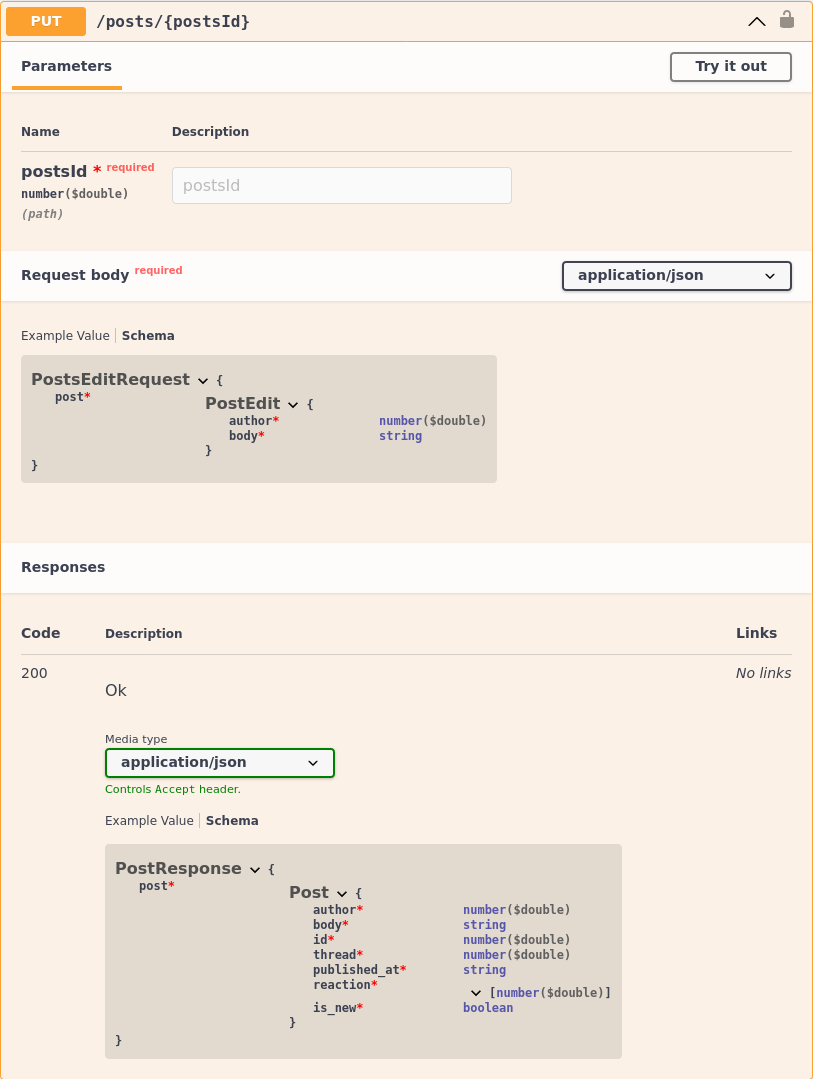
\includegraphics[width=\textwidth]{assets/img/swagger-ui}
\caption{The visualization of the post edit endpoint by Swagger \acrshort{UI}}
\label{fig:swagger-ui}
\end{figure}

After the `swagger.json` definition file is generated on the backend, the `swagger-codegen`~[@swagger-codegen] tool can be used to generate respective code on the frontend:

~~~ JavaScript
public postsEditSingle(body: PostsEditRequest, postsId: number): Observable<PostResponse>;
~~~

Internally, this function will handle authorization and possible exceptions so that the developer can use it as a regular function without worrying about its inner workings.

### Drawbacks and advantages

Because the definition of the \acrshort{API} is stored within a separate project, this could in the future lead to a de-synchronization between the definition of the \acrshort{API} and the backend code itself. Nevertheless, this threat would be present in some form unless the `swagger.json` can be generated directly from the backend code. If no technology like OpenAPI is used, then every time a backend endpoint changes, all frontend usages of such endpoint have to be manually reviewed. The separate project is a compromise, which minimizes the risk of de-synchronization by using a simple to use syntax for the backend developers and easy changes implementation by regenerating the code from the Swagger definition for the frontend developers.

## Docker container

The only public instance of the \acrshort{KSI} backend is for the production environment. The second instance, created for testing purposes, is only available from inside the faculty network, which makes it inappropriate for comprehensive testing by all \acrshort{KSI} organizers. Not every organizer is also a student of the \acrshort{FI}. This makes the need for another backend instance obvious. Furthermore, being able to create multiple instances for local testing during development efficiently decreases the chance of more significant issues because of their local scope.

The backend project itself has only a few external dependencies -- except for Python 3 environment, it needs a \fnurl{`isolate`}{https://github.com/ioi/isolate/} project executable for sandboxing untrusted participants' code and a database to connect to. Selecting a base Docker image of Python 3 based on \fnurl{Debian buster}{https://hub.docker.com/_/python} makes it possible to create an environment similar to the \acrshort{KSI} production server. Almost every required modification to the backend project can be done directly inside the \fnurl{Dockerfile}{https://github.com/fi-ksi/web-backend/blob/master/.docker/Dockerfile}, namely:

- because `isolate` is not available as a Debian package, it must be compiled manually. The Dockerfile downloads the built version from my personal Debian package repository
- for easier manipulation with the database, an SQLite database file will be used instead of the MariaDB server used on production. This decision has a few implications:
    - the SQLite database backend does not automatically convert data types, so some source code patches were needed to fix data types passed to the database
    - SQLite does not fully implement all SQL language features, for example `CURRENT_TIMESTAMP + INTERVAL 1 SECOND` has to be replaced with `datetime("now", "+1 seconds")`
- the backend server needs to be accessible from the Docker container's IP address, while the default settings are to be accessible only from localhost
- `isolate` requires the `/etc/` directory to be bind-mounted as `/opt/etc`, which is not possible inside a Docker container unless the container is started in a privileged mode
- the default starting script, which launches the server as a background daemon, needs to be replaced with a different container entry point that stays in the foreground, which helps start the container in an interactive mode

The data of the backend server, together with the SQLite database file, are kept externally and are only bind-mounted to the container so that rebuilding the docker image does not erase them. Only when the container's entry point is executed the data is mounted into the appropriate location. To prevent insufficient permission when accessing the data by the unprivileged `ksi` user inside the container, the actual owner is masked by using the `bindfs` tool. The `bindfs` is also used to bind-mount `/etc/` to `/opt/etc` to bypass higher permission requirements for the Docker container. 

Because the container is running in a privileged mode with shared `/dev/fuse` for the `bindfs` tool, it is currently undesirable to execute the production server inside the container, as it may pose a security risk. On the other hand, the container is entirely suitable for usage during the development of the frontend application. Furthermore, the whole docker container can be packaged inside a `.tar` file and then transferred to another machine, making the process of creating another backend instance faster. This feature was used when deploying a temporary \fnurl{testing server}{https://ksi.ahlava.cz/api/years}, which is available for all \acrshort{KSI} organizers and is running inside the docker container.

\end{markdown*}

\mdchap{Final web application}

This chapter describes the implementation of the new web application frontend itself. The first part of this chapter analyzes the application architecture and code structure while highlighting specific decisions made during the development, while the second part is focused on the design of the user interface presented directly to the user.

Next, the modularity of the new web frontend is demonstrated in the example of the second deployed instance, and the approach to introducing historic \acrshort{KSI} tasks to the new web application is described. Finally, the new frontend is evaluated based on feedback received from its users.

## Application architecture

\begin{figure}
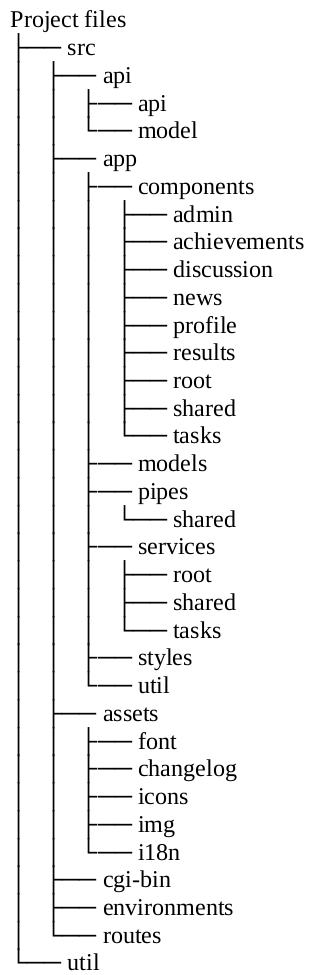
\includegraphics[width=.3\textwidth]{assets/img/file-tree}
\caption{The directory tree of the new web application project}
\label{fig:file-tree}
\end{figure}

### Project's directory tree

The project's file tree is a crucial architecture design choice as it will impact the entire project. Because the Angular framework has a set directory structure~[@angular-tutorial], this project expands upon it to make it as easily accessible to new developers as possible (\autoref{fig:file-tree}). The project's root directory contains two main subdirectories -- `src` with the source code of the application and `util` for helper scripts that perform automatic tasks.

#### Source directory

Same as Angular defaults, the source directory contains the `app` subdirectory for web application code, `assets` for holding static files that are not a direct part of the code and `environments` that define constants specific for every instance (for example URL for the backend server). The `api` directory holds all code generated by the `swagger-codegen` tool (\autoref{chap:swagger-codegen}). Inside the `cgi-bin` directory is located the script required for automatic deployment (\autoref{chap:autodeploy}).

The application files are split into subdirectories based on their Angular type (`component`, `model`, `pipe` and `service`). Next split is upon their module (`achievements`, `discussion`, `news`, `profile`, `results`, `root`, `tasks` and `shared`). The modules (except for module `shared`) are respective to their relative application path -- e. g. components that are inside the `news` module will have a path starting with `/news/`. This splitting is done both for more rational file placement and faster loading times by utilizing lazy modules (\autoref{chap:faster}). The shared module contains items shared across multiple other modules, for example, the loading spinner, which is included on almost every page. Models, services and pipes all contain in their root an `index.ts` file, which exports all their members from their subdirectories for possible future easier refactoring.

The `styles` directory contains global variables to be imported in components, \fnurl{SCSS mixins}{https://www.koderhq.com/tutorial/sass/mixin/} for common style adjustments, color palette definition and theme variables (\autoref{chap:theming}). The colour palette is generated as shades from \fnurl{internal \acrshort{KSI} colours}{https://github.com/fi-ksi/grafika}. To make the colour replacement for other projects derived from this thesis as simple as possible, almost no other colours are used in the entire application, with the only exception being colours retrieved from the project's third-party dependencies.

Lastly, inside the `util` are defined static utility classes that are not part of a single Angular type but are still used in multiple of them. These utility classes handle tasks like rewriting an asset URL retrieved from backed for the current web application to the location of the same assets inside the new application.

#### Utilities directory
\label{chap:utils}

The project's root `util` subdirectory contains shell scripts for automatizing tasks. The \acrshort{PWA} (for an explanation, see \autoref{chap:faster}) requires the icon to be of the exact size, while the new web application uses an \acrshort{SVG} icon, the `gen-icons.sh` script takes the main \acrshort{SVG} icon and converts into multiple icons with a fixed resolution for the \acrshort{PWA}. The `gen-api.sh` script automatically downloads the correct version of `swagger-codegen` tool (\autoref{chap:swagger-codegen}) and executes it to generate \acrshort{API} code inside the `src/api` directory. It also attempts to fix the code that was generated incorrectly -- for example, by correcting the type of recursive array or by unescaping HTML text (`'&lt;'` is replaced for `'<'`; `'&gt;'` with `'>'`) and modifying incorrectly typed function for downloading a file from the backend.

The `gen-scss-theme.sh` is further explained in \autoref{chap:theming}, `gen-changelog.sh` in \autoref{chap:changelog}. All utility scripts have their respective alias inside `package.json` file for convenience -- `npm run` `gen.icons`, `gen.api`, `gen.theme` and `gen.changelog`. 

### Theming
\label{chap:theming}

The new web applications supports switching between so-called light (\autoref{fig:light-mode}) and dark (\autoref{fig:dark-mode}) modes. Internally, the modes are implemented as \acrshort{CSS} variables, which get overridden by adding a `theme-dark` class to the page's `body` element. All \acrshort{CSS} variables are defined inside `src/app/styles/theme.scss` with the name of their main occurrence, though they are reused as much as possible to minimize required changes for other projects derived from this thesis. The \acrshort{CSS} is not to be used directly in other styles; rather, they are used as an input for the `gen-scss-theme` utility script (\autoref{chap:utils}), which wraps all \acrshort{CSS} variables as SCSS variables at the end of the file. The main advantage of this approach is that if a variable was removed or renamed, then an error during compilation will be shown for a missing SCSS variable instead of silently ignoring the missing \acrshort{CSS} variable.

\begin{figure}
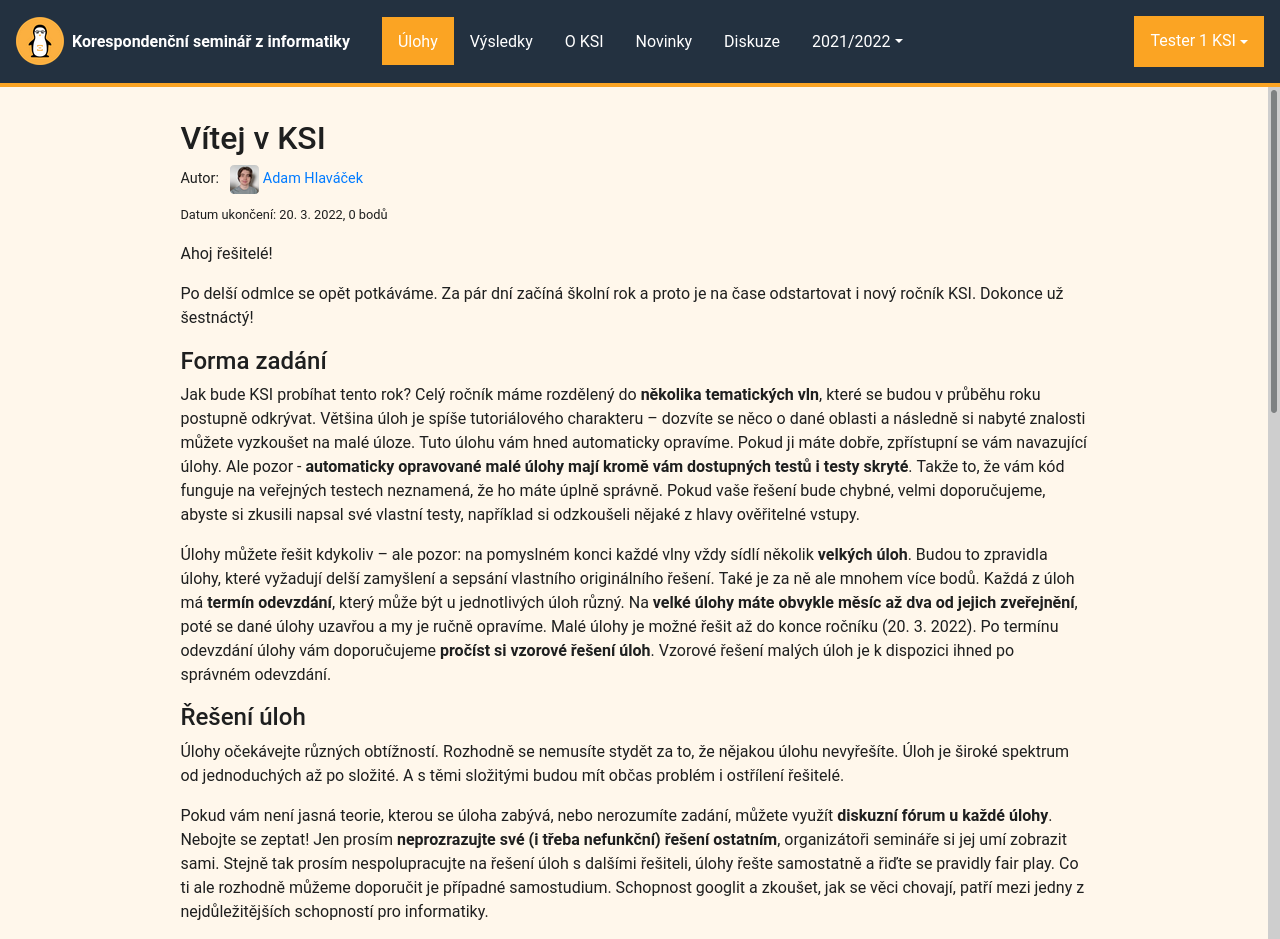
\includegraphics[width=.8\textwidth]{assets/img/light-mode}
\caption{Task page in a light mode}
\label{fig:light-mode}
\end{figure}

\begin{figure}
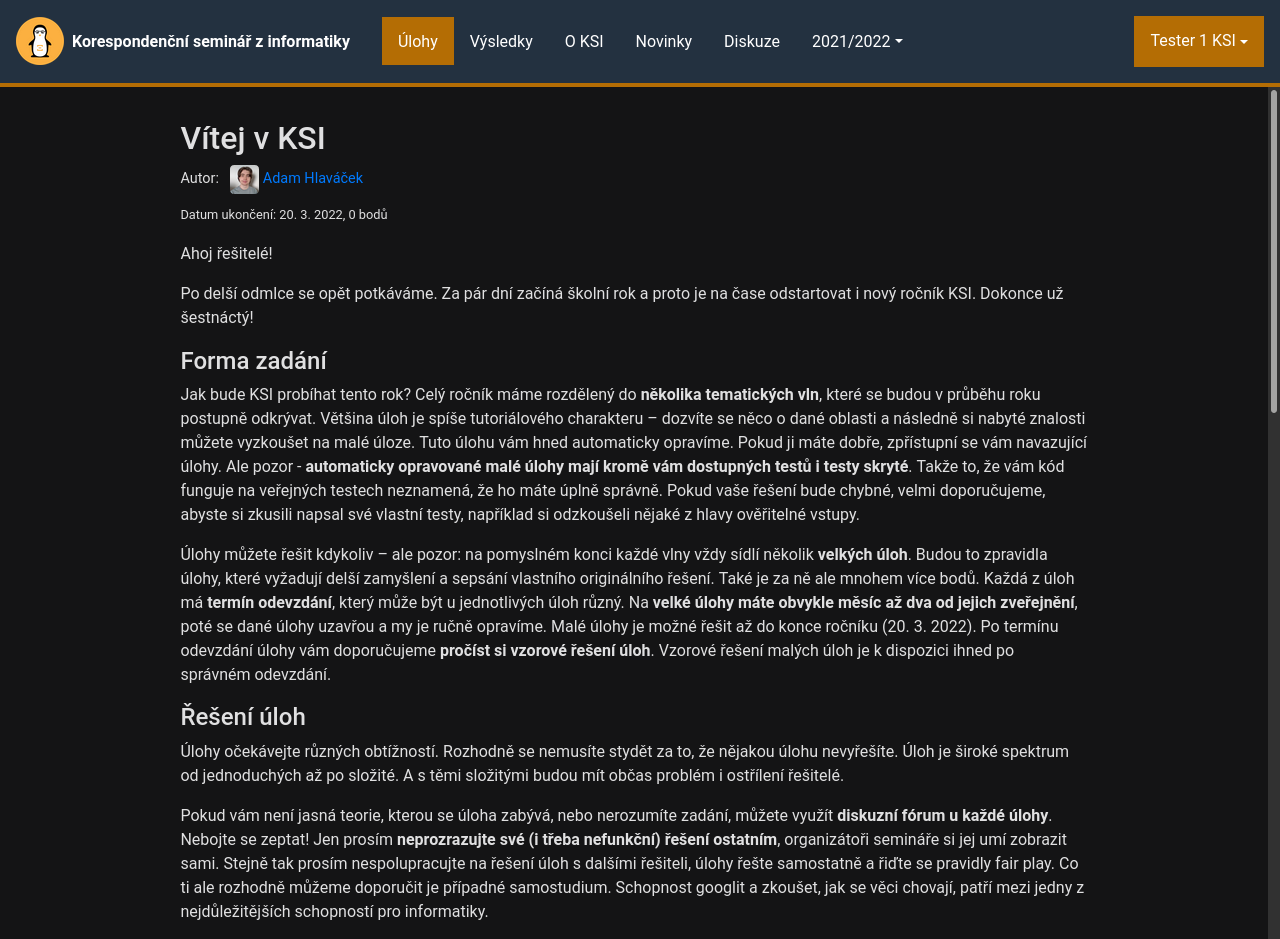
\includegraphics[width=.8\textwidth]{assets/img/dark-mode}
\caption{Task page in a dark mode}
\label{fig:dark-mode}
\end{figure}

### Internationalization
\label{chap:translations}

To make translations of this project or adjustments of texts for other projects derived from this thesis as simple as possible, almost all text strings are separated from the main code, the only exception to this rule being the page titled About \acrshort{KSI}, which is expected to be replaced entirely with another page in other projects. The rest of the texts are placed inside a \acrshort{JSON} file `assets/i18n/cs.json`. This file has a dictionary structure, in which are the string referenced by their qualified name -- for example, given the following `en.json` structure and Angular HTML component template

```JavaScript
// en.json
{
	"main-page": {
		"title": "Example title"
	}
}

// component template
<h1>{{'main-page.title'|translate}}</h1>
```

the result on the results page will be `<h1>Example title</h1>`. Also, by having all texts inside a \acrshort{JSON} file, we can switch translations and target language by simply providing another \acrshort{JSON} file during the application's runtime, as the `translate` pipe is implemented as an RxJS observable. Furthermore, because the qualified name format is used, it is possible to create gender-specific texts by appending e. g. `.male` or `.female` to the name, practical for the Czech language.

In addition to translating the texts inside the application, the path names are also localized. However, this localization is only applied during the application's build process. The pathnames are defined inside the `src/routes` directory, where files implement the `IRoutes` interface from the project's models. Furthermore, referencing routes through this interface rather than by pathname makes it possible to rename application routes without multiple changes to application components.

### Automatic deployment
\label{chap:autodeploy}

When a process of automatic deployment is triggered, the web application is automatically built and then released on the selected instance, be it production, testing or other. The usage of automatic deployment decreases the developer's work required to release the newest version of the application. It takes care of repetitive steps and can be triggered, for example, by a simple push to a named git branch inside the project's repository. The process can also be safer than manual deployment because software tests can be a part of the automatic process. If some of the executed tests fail, the deployment can be rejected. This assures that no version that does not pass the tests will be released to a production environment.

#### GitHub Actions

Because both current and new web applications exist as projects on GitHub, they can take advantage of the GitHub Actions feature. The GitHub Actions are a sequence of steps and commands (e. g. to create a new release of a GitHub project or to execute Bash script) that are to be executed when a specific event occurs -- most often a push to a particular git branch. They are defined as \acrshort{YAML} files inside the project's `.github/workflows` subdirectory and can reference other projects as modules or use variables and secrets set in the GitHub repository settings.

#### Current automatic deployment process

Currently, when a push action is performed on one of the watched branches, an automatic process is triggered in the form of GitHub action. The process consists of building the web application and then copying the distribution files over an \acrshort{SSH} connection to the author's home directory inside the \acrshort{FI} network. From there, the files are once again copied to the target server. The distribution files cannot be copied to the target server directly because of security precautions from the \acrshort{FI}, which block \acrshort{SSH} traffic to the \acrshort{KSI} servers coming from outside the \acrshort{FI} network. The main disadvantage of this process is that it requires an active student account. Also, no tests are executed during the deployment process, and an incorrect code can result in production downtime.

#### New deployment process

The new automatic deployment process is also triggered upon a push to a watched branch. First, all requirements are installed, and then the application is built for the selected environment. During the build process, the code is checked for type safety, and if any typing error is found, the deployment is cancelled, and the user whose push has triggered the process is notified about its failure. A GitHub project release containing the file `built.tar` with complete distribution files is created if the build process is successful. The file `build.tar` has a unique address, which is passed to a deployment \acrshort{CGI} script (`src/cgi-bin/dist-update.sh` inside the project's source tree, this script must be manually saved on the target server before the first automatic deployment) by calling it over \acrshort{HTTP}. The notified \acrshort{CGI} script then downloads the `build.tar` release and overwrites current files by the content of the `build.tar` package. A final step of the build process is to delete the created temporary release.

This new deployment process does not rely on any specific person to participate. The only requirement is the existence of the called \acrshort{CGI} script on the target server. To mitigate security concerns about downloading an untrusted `tar` file and blindly replacing its own files with its content, the \acrshort{CGI} script contains various protection methods. Foremost, the script is supposed to be accessible only when a correct authorization is performed to the webserver beforehand, which, together with a strong password (saved as project's secret inside GitHub's project settings), will mitigate most attack attempts, as the webserver will handle those and the script will not be executed. If the attacker was to gain access by guessing the correct password, then the script itself will check that the owner and repository of the `build.tar` match with expected values and, if not, refuse to perform the action. Finally, the \acrshort{CGI} script is executed in a sandboxed environment with write access only to the distribution files to prevent accidental file modification.

### Automatic changelog generation
\label{chap:changelog}

To keep the users of the web application informed about development progress, a changelog dialogue was shown whenever a change has been made since the user's last visit (\autoref{fig:changelog}). The changelog is generated automatically based on git commits history. This is possible due to respecting Conventional Commits specification~[@conventional-commits], where commits have a structure similar to `feat(category): description` or `fix(category): description`. Parsing such commit messages from git history is a trivial task, consequently making generating an automatic changelog practically effortless. The changelog is generated on build time or by manually executing the `util/gen-changelog.sh` script. Regenerating the changelog also updates the application version number.

\begin{figure}
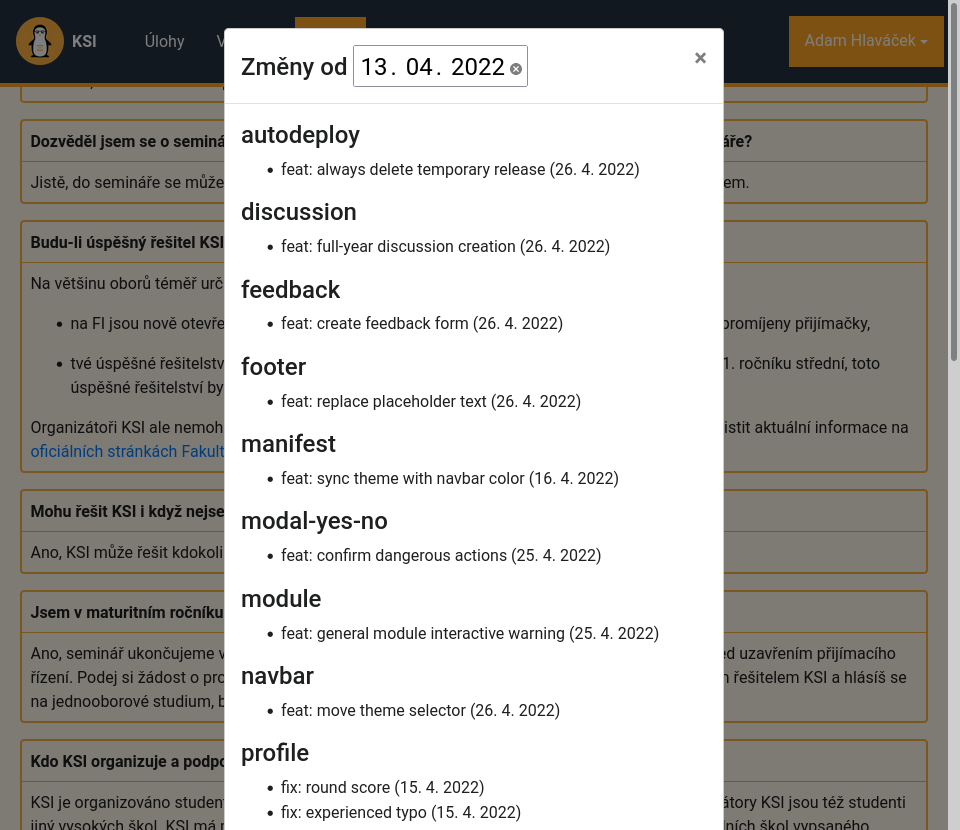
\includegraphics[width=\textwidth]{assets/img/changelog}
\caption{A changelog dialogue with recent changes}
\label{fig:changelog}
\end{figure}

### Login status and theme synchronization

Whenever the user changes the preferred colour theme or logs in or out, the information about this action is synchronized across all opened tabs through \fnurl{`BroadcastChannel`}{https://developer.mozilla.org/en-US/docs/Web/API/BroadcastChannel} API. This feature dramatically improves \acrshort{UX} in such cases when the user opens multiple tasks that require logging in at once without logging in. By simply entering user's credentials in one of the opened tabs, the status will be propagated across all tabs without any additional input from the user.

### Improved loading times
\label{chap:faster}

All modules (except for the `shared` module) are imported as Angular lazy modules~[@angular-lazy] to improve loading times. This assures that the application will load the minimal subset of code required to render content on the first load. Additional code from different modules is downloaded automatically when the user requests it, typically when navigating to another subpage. Furthermore, Angular provides a simple way to convert the application into a so-called Progressive Web Application, PWA for short. PWA relies on a Service worker technology that works as a proxy for all network requests made by the application~[@angular-pwa]. As such, it can intercept the requests and return a version saved in the cache instead of passing it through to the server. Most modern browsers support service workers, so the web application is cached automatically after the first load. The subsequent call will be returned from the cache, making loading pages instantaneous. In the background, the service worker checks if the application's code was changed. If so, the new version is then silently downloaded and applied upon the next load of the application, making the transition between versions seamless. In the future, this behaviour could be a prerequisite for a fully offline available \acrshort{KSI} web application. However, it would require backend modification and possibly break its compatibility with the current web application.

## UI Design

During the development of the application, the following principles were maintained:

1. everything has to be accessible on a mobile phone
2. provide a unique link whenever possible
3. prefer asynchronous operations
4. cache mainly static but frequently accessed information

Because the current web design still appears sufficient nowadays, the overall new look of the web page is similar -- the colour pattern was generated as shades defined from primary \acrshort{KSI} colours, and all icons were reused from the current web application.

### Landing page

The landing page is referenced on every propagation media and, as such, is the first element of the \acrshort{KSI} web application that possible participants will most likely see. The current landing page~( \autoref{fig:welcome-curr}) uses a signification portion of space for large icons and long text blocks. It also presents a clickable button in the middle of an image, which is a disturbing design pattern. To address these issues, the new landing page~(\autoref{fig:welcome-new}) splits the content into two rows so that the newest information is visible without any scrolling required. The longer texts have been hidden behind the carousel, which is shown when the user clicks on one of the key \acrshort{KSI} points in the middle of the screen.

A second most notable design choice that differs from the current web application is the width and colour of the navigation bar. In the current version, the navigation bar is located near the middle, whereas the new application covers the entire width of the screen with unified colours. This approach gives a more breathable feel and makes it easier to scale on different resolutions.

\begin{figure}
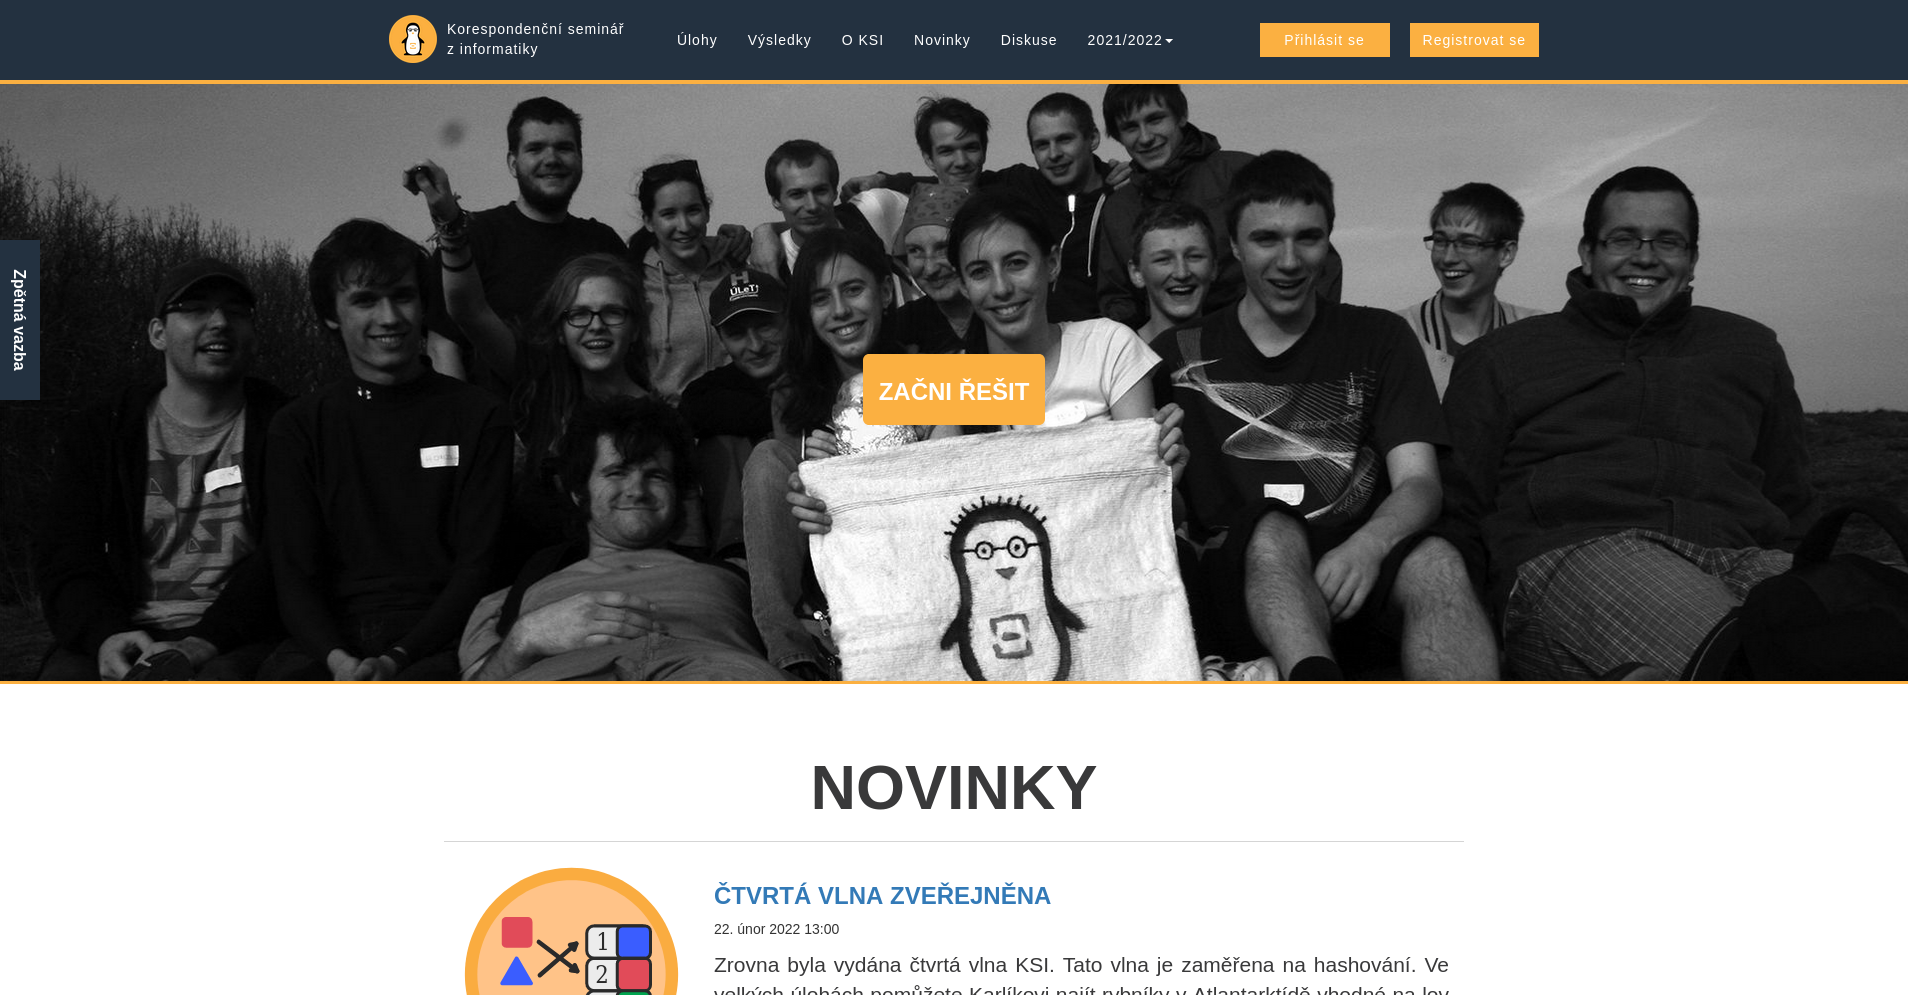
\includegraphics[width=\textwidth]{assets/img/welcome_curr}
\caption{The current \acrshort{KSI} landing page on desktop}
\label{fig:welcome-curr}
\end{figure}

\begin{figure}
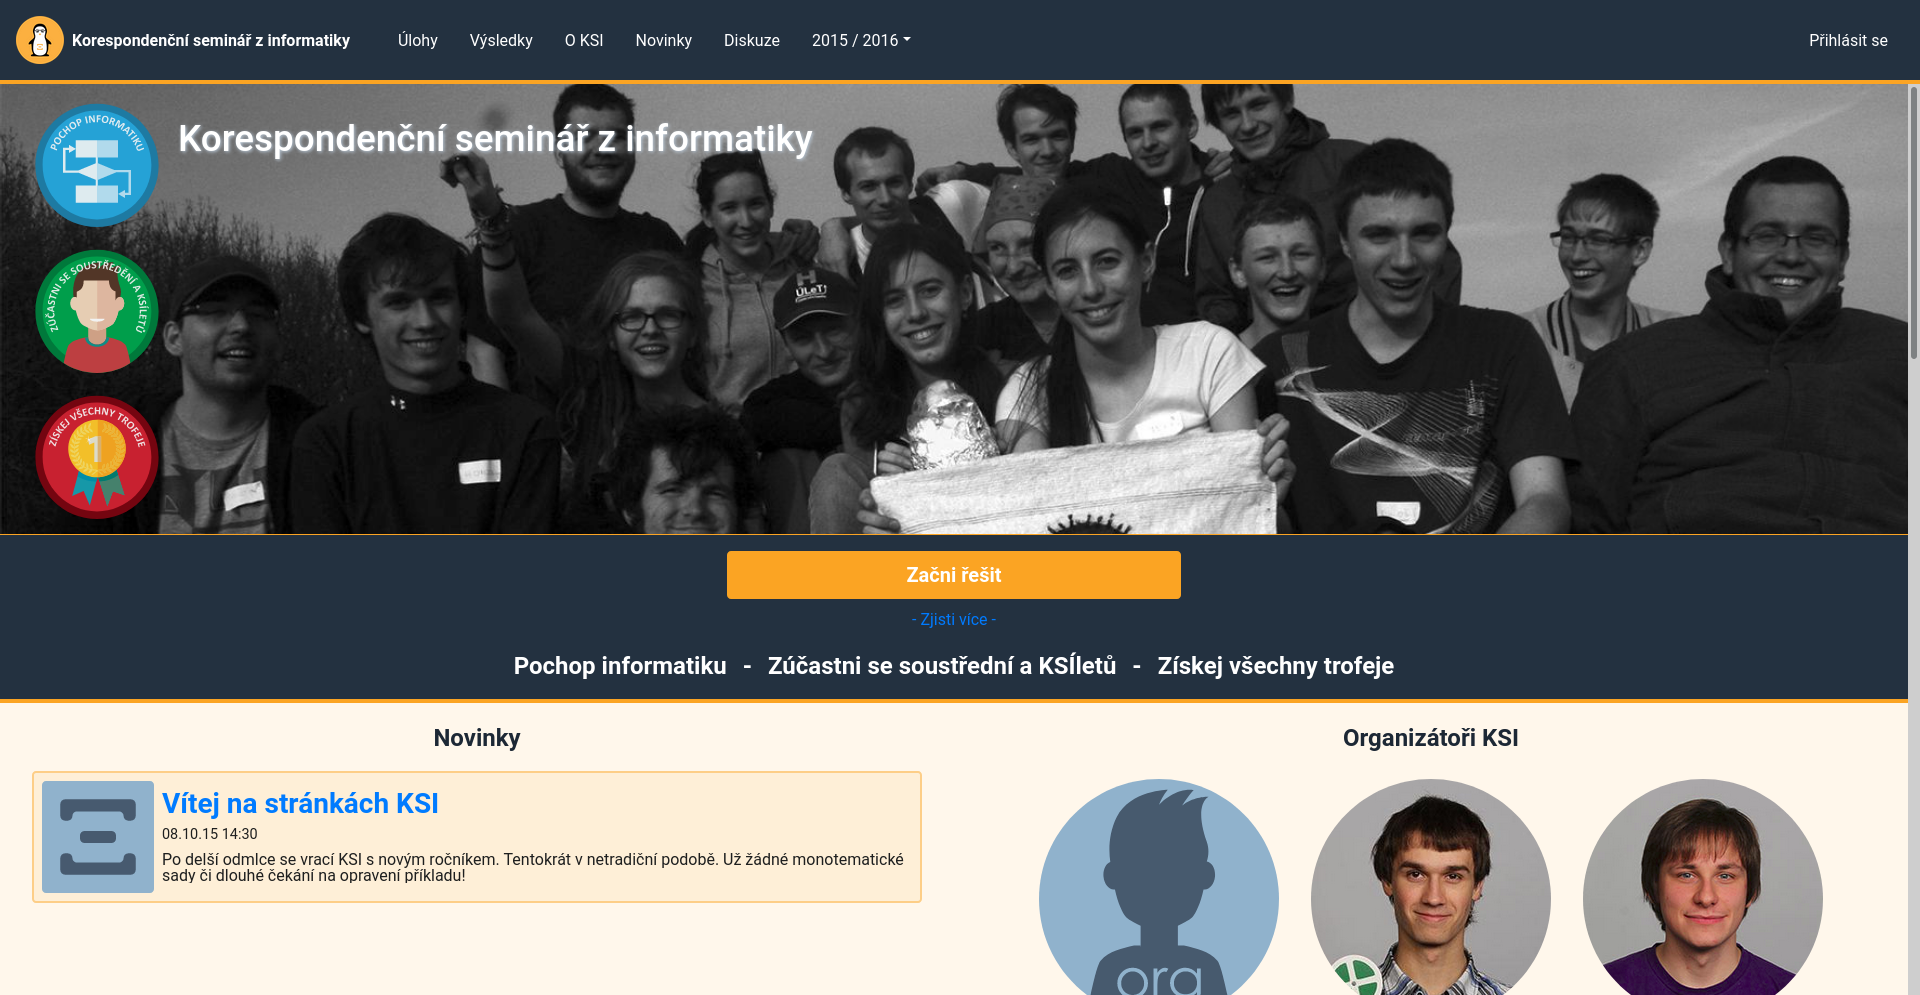
\includegraphics[width=\textwidth]{assets/img/welcome_new}
\caption{The new \acrshort{KSI} landing page on desktop}
\label{fig:welcome-new}
\end{figure}

### Tasks graph page

The main point of \acrshort{KSI} is a page with all tasks available to participants. The tasks are presented in the form of a directed acyclic graph, which can precisely represent which tasks are required to be completed before proceeding to the next ones.

The current version of the web frontend (\autoref{fig:graph-curr}) shows a legend explaining the different graph node colours on the left, which moves the whole graph slightly to the right side. Moreover, the graph could get more complicated and unclear as new tasks are added with a year's progress. The new web frontend (\autoref{fig:graph-new}) tries to take maximum advantage of the available page width. This is done by moving the legend into a modal dialogue (\autoref{fig:graph-new-settings}) accessible by a help button in the top right corner of the page. Given that the legend is mainly used by only new users of the \acrshort{KSI} web application, there is a little need to keep it visible all the time. Furthermore, to increase the clarity of the task graph, the user can turn splitting the whole graph into multiple smaller graphs by grouping them into their thematic waves (\autoref{fig:graph-split}). In this mode, the user can then keep open only the relevant parts of the graph, presumably only the currently active \acrshort{KSI} task wave.

Though, the most notable change can be seen when using the \acrshort{KSI} web application on a mobile phone (\autoref{fig:graph-mobile}). In the current version, the graph on the mobile is too narrow to fit, which results in multiple tasks overlapping. This makes it nearly impossible to open the correct task. Instead, a special graph presentation mode was created in the new web application. In this mode, the tasks are shown in the mode of a list, where tasks required to be completed before other tasks can be unlocked shown first. This mode lacks information about different graph branches as seen on the desktop version but provides a viable compromise to usability on a mobile phone.

In the spirit of the third followed principle, all tasks in all modes are now rendered as HTML anchor points instead of clickable canvas as in the current version. The advantage of this approach is that now every task can be quickly located by using the search function of a web browser, and multiple tasks can be opened in a new tab by pressing the middle button on the mouse or saved for later without having to be opened one at a time.

\begin{figure}
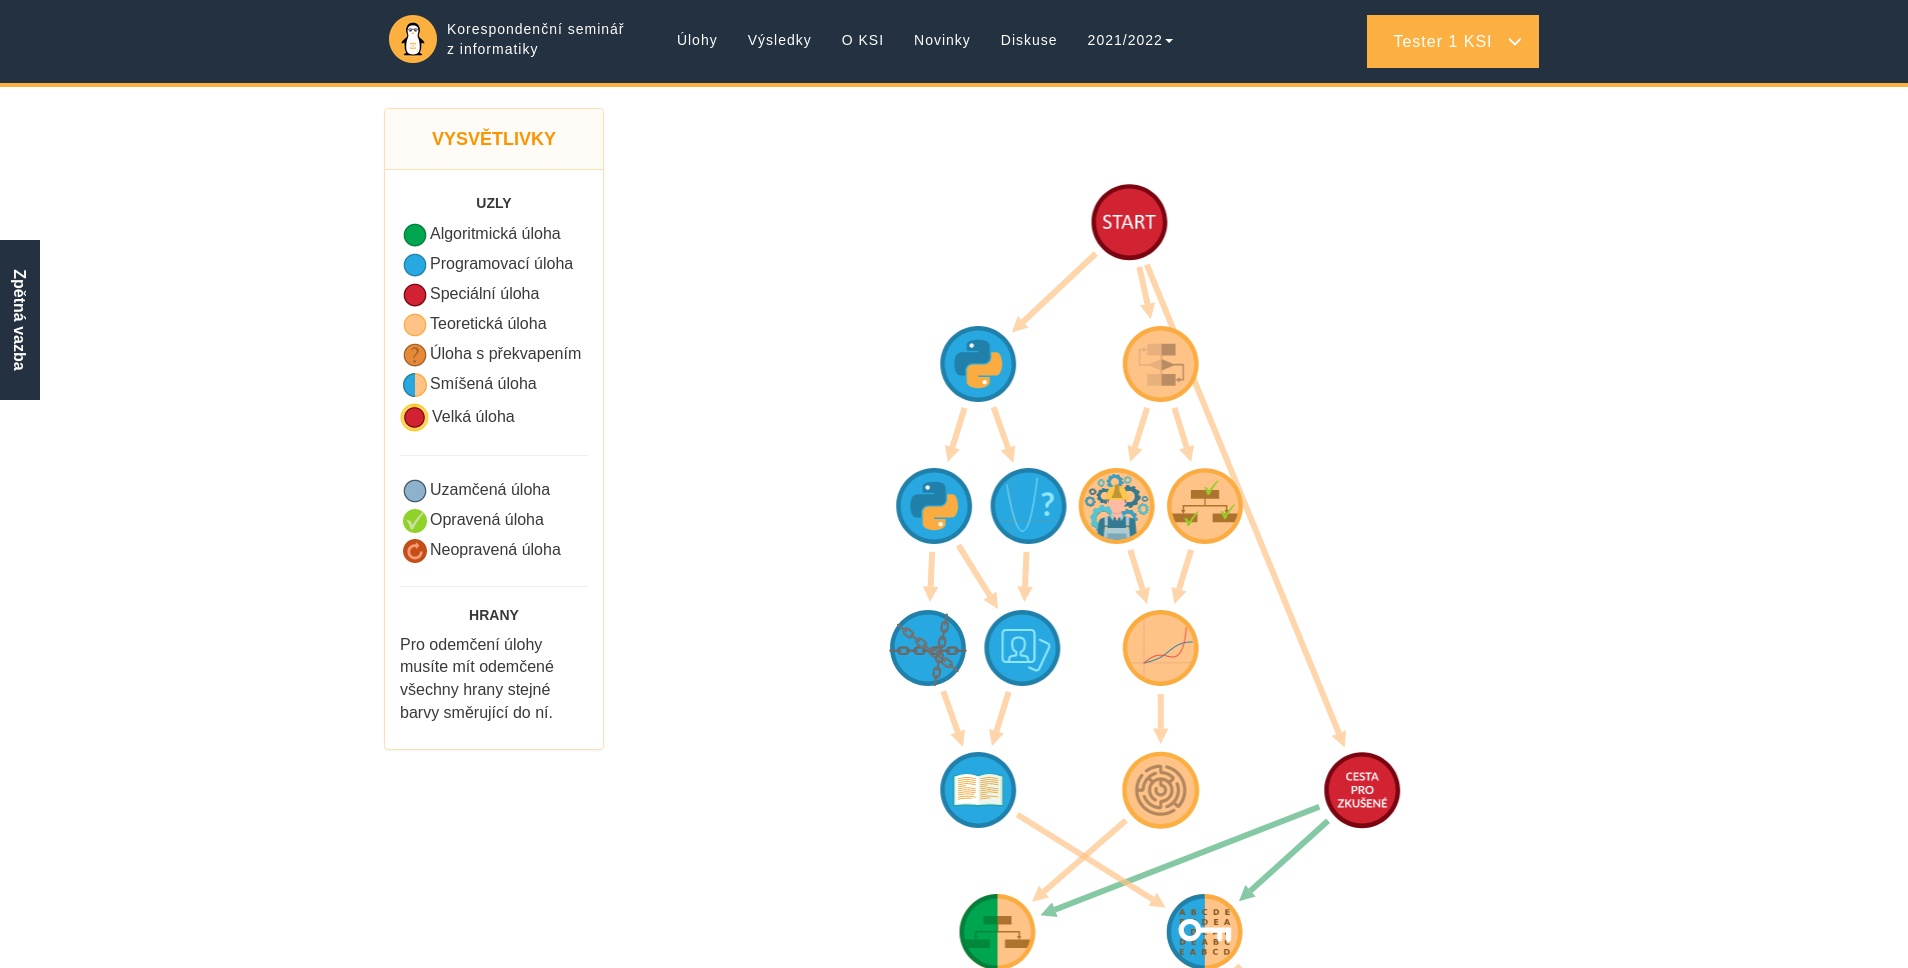
\includegraphics[width=\textwidth]{assets/img/graph_curr}
\caption{The current task graph}
\label{fig:graph-curr}
\end{figure}

\begin{figure}
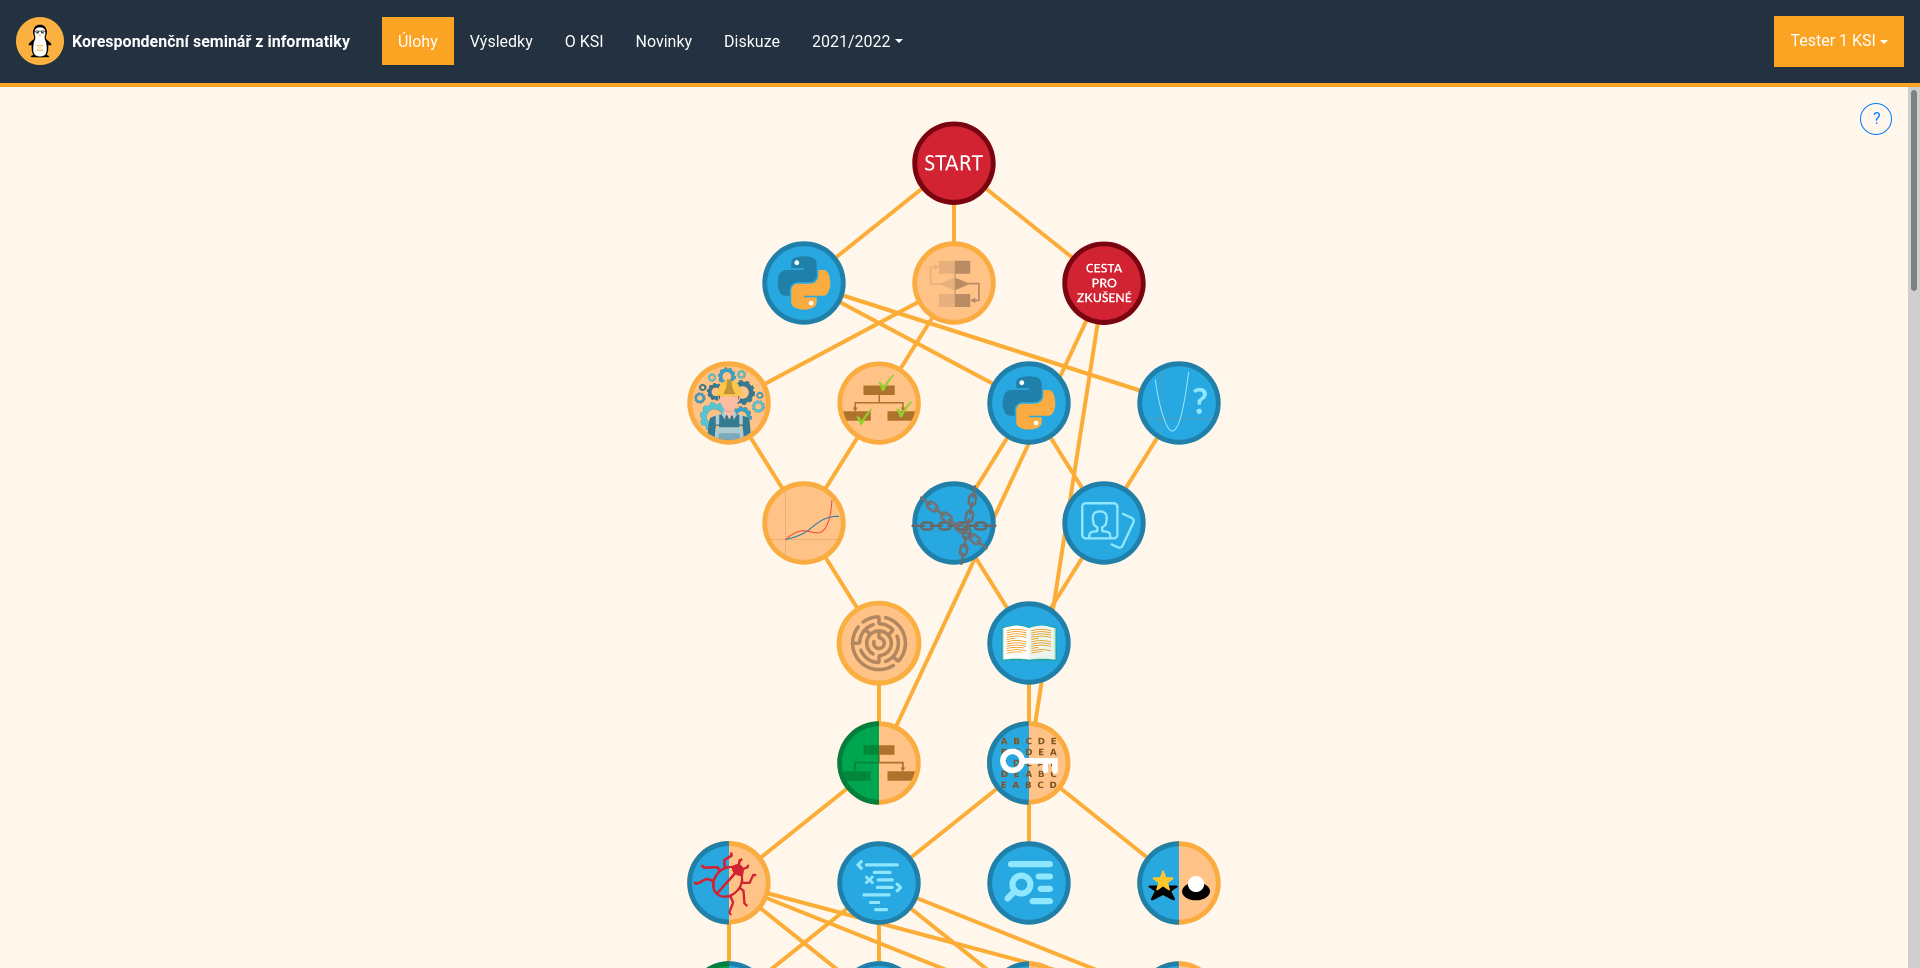
\includegraphics[width=\textwidth]{assets/img/graph_new}
\caption{The new task graph}
\label{fig:graph-new}
\end{figure}

\begin{figure}
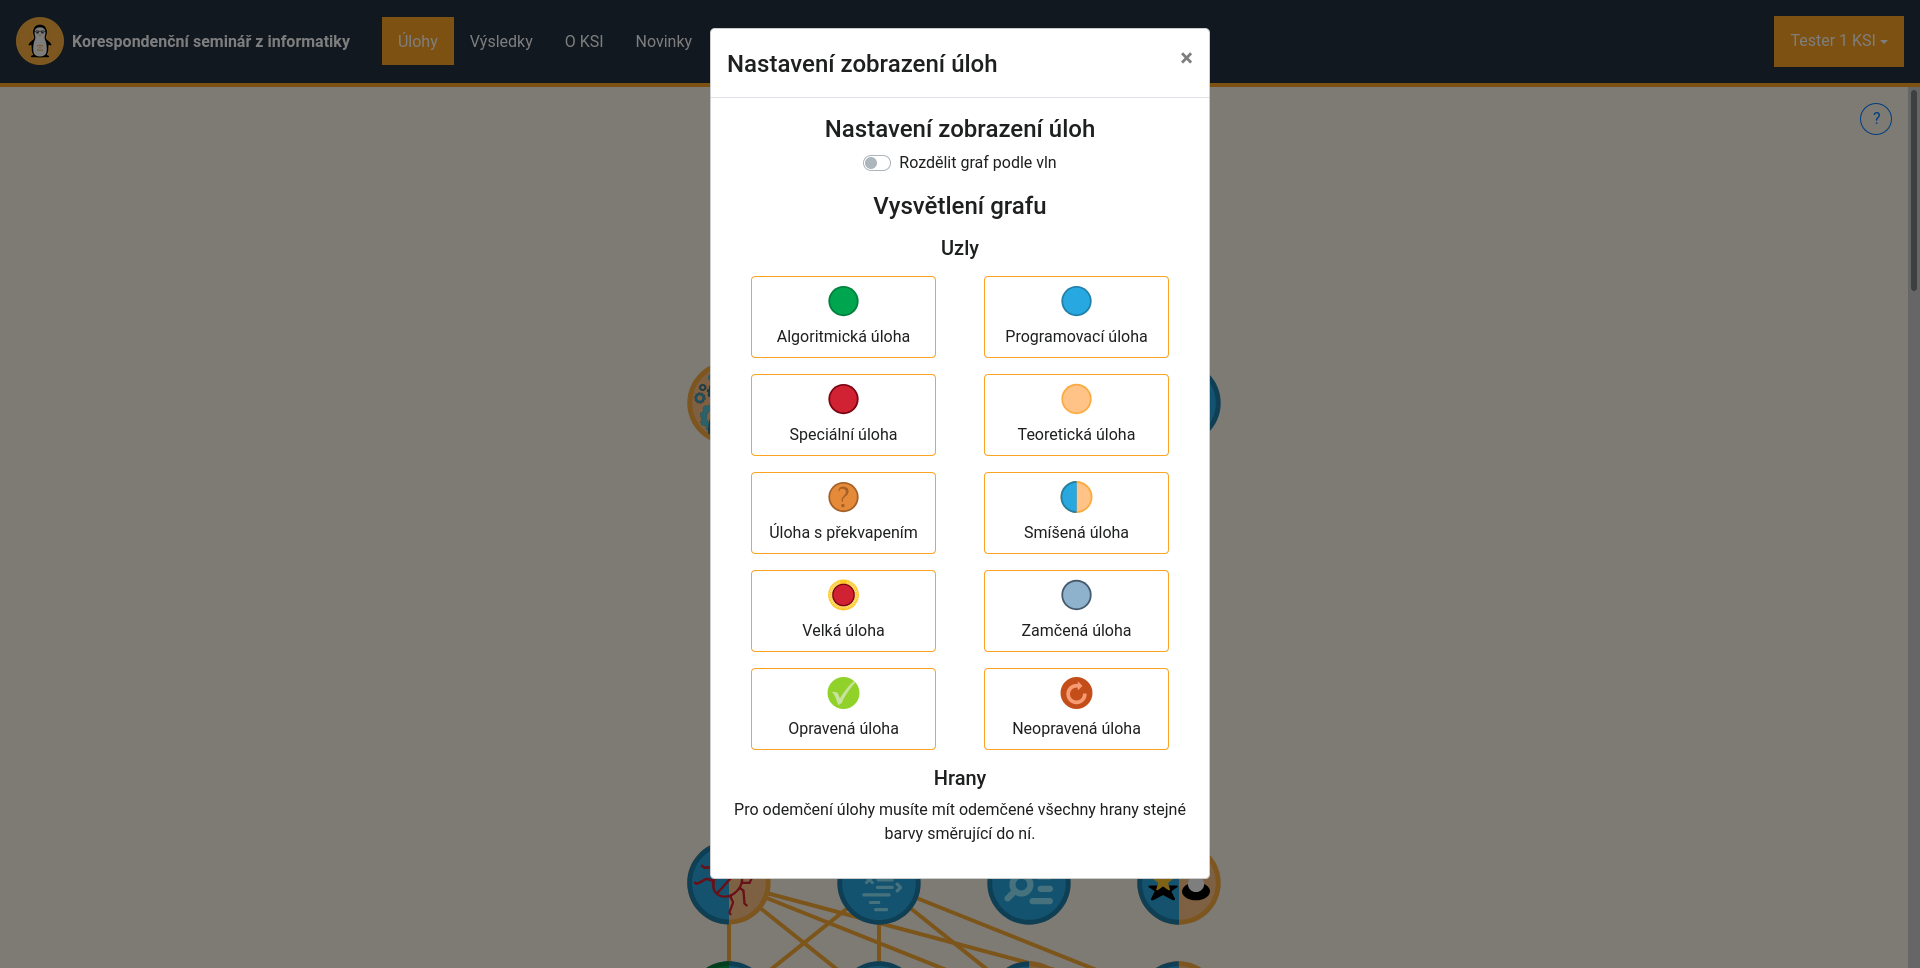
\includegraphics[width=\textwidth]{assets/img/graph_newsettings}
\caption{The settings of the new task graph with a legend}
\label{fig:graph-new-settings}
\end{figure}

\begin{figure}
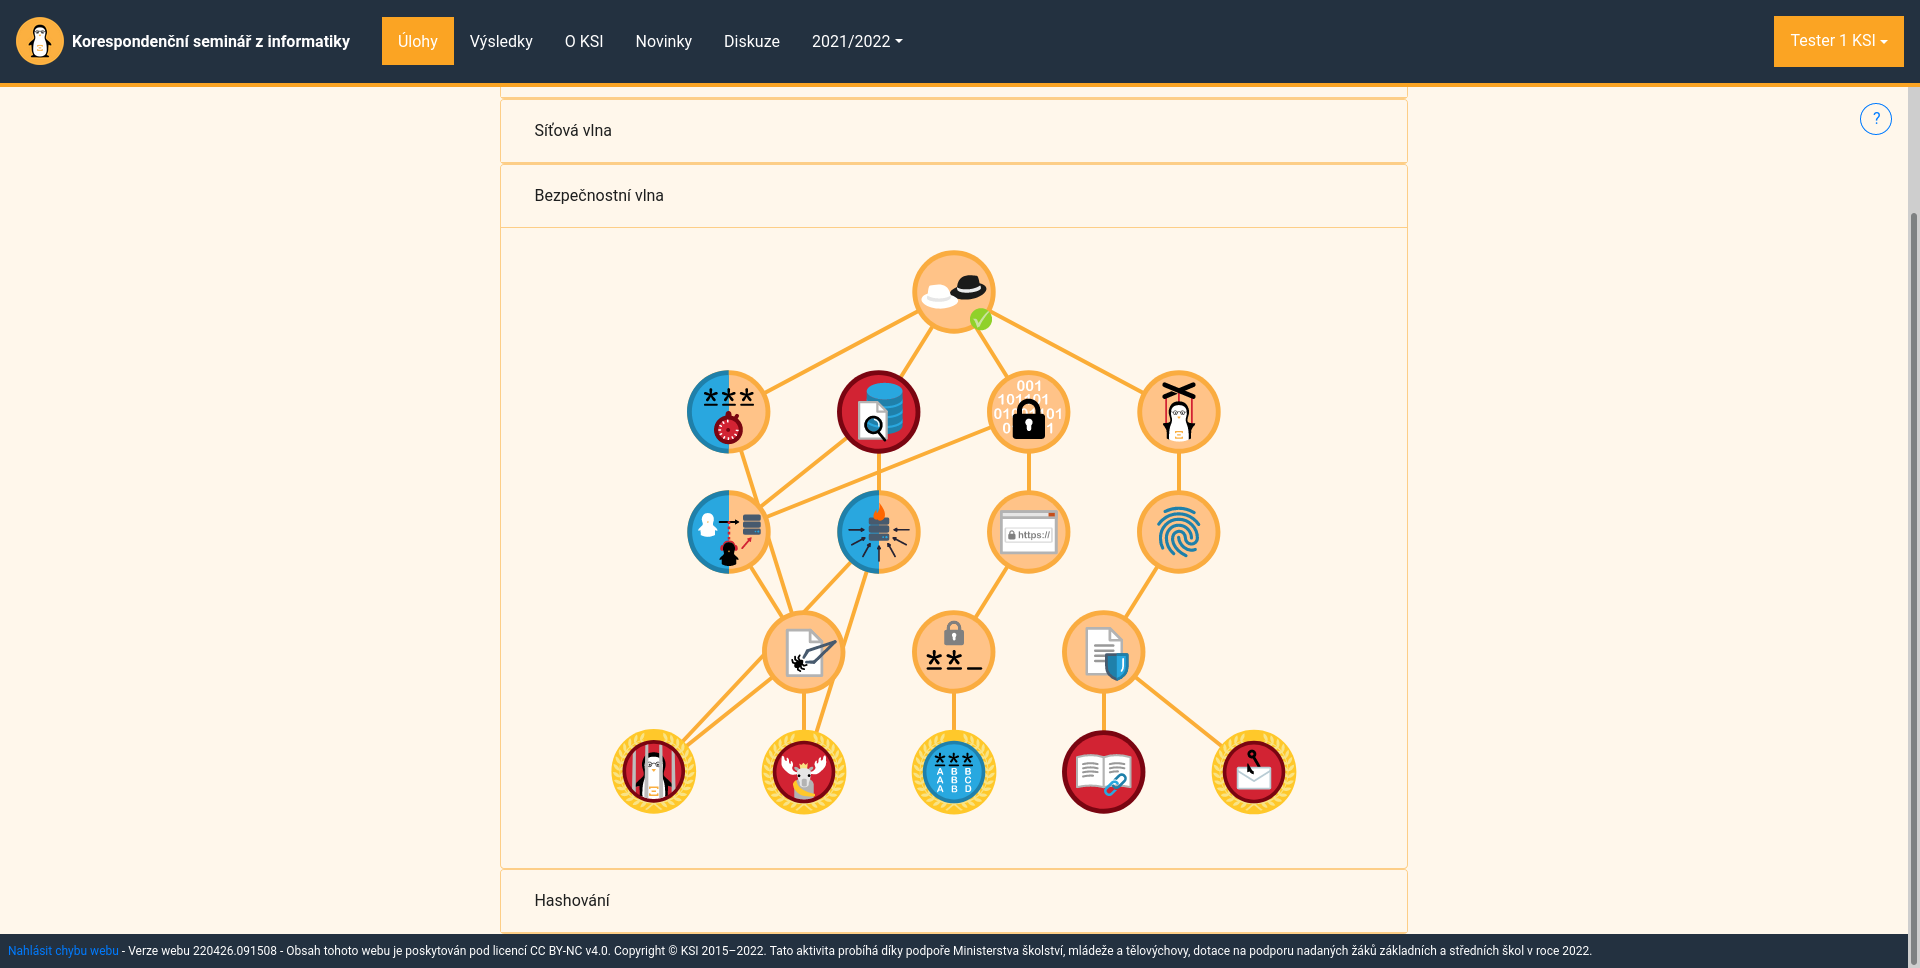
\includegraphics[width=\textwidth]{assets/img/graph_split}
\caption{The task graph, when split into wave groups}
\label{fig:graph-split}
\end{figure}

\begin{figure}
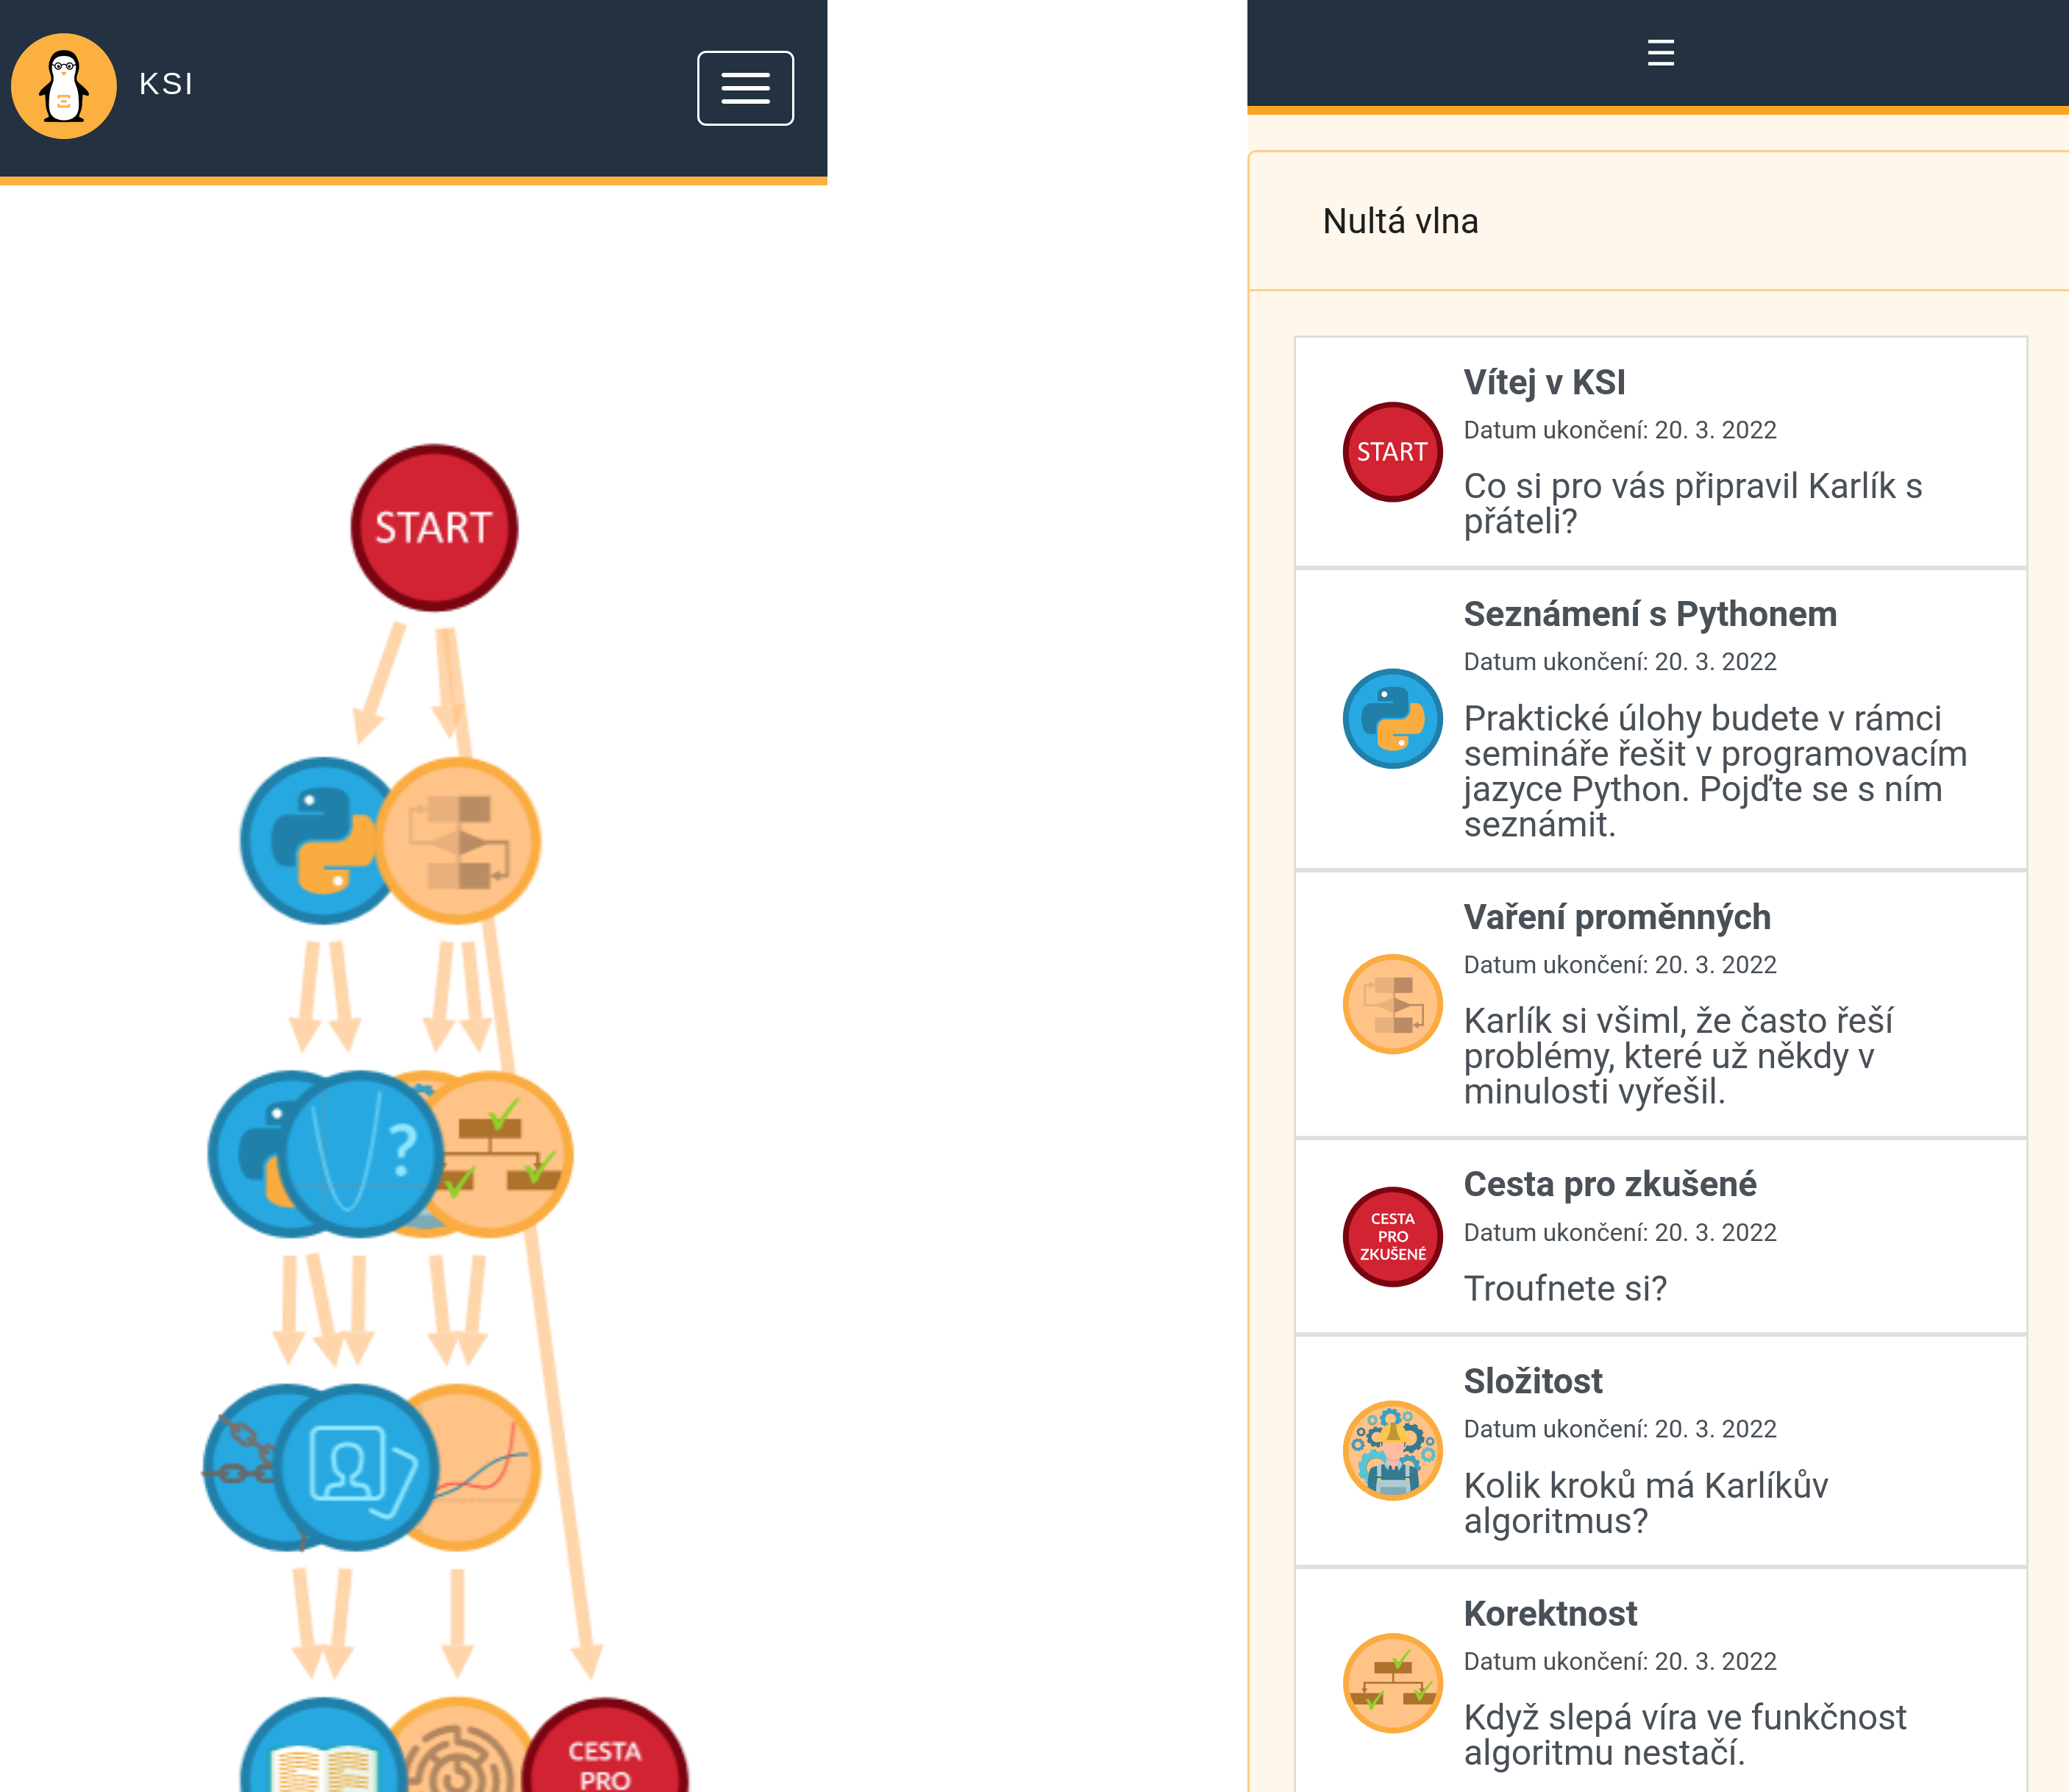
\includegraphics[width=.5\textwidth]{assets/img/graph-mobile}
\caption{The task graph when seen on a mobile phone (current left, new right)}
\label{fig:graph-mobile}
\end{figure}

### The task page

The functionality of a \acrshort{KSI} task page remains almost unchanged. Mainly, design modifications were made. In the current version (\autoref{fig:task-curr}), the task has a section selection in its begging, where it may feel disruptive and complicated. Most of the time, the participant does not need to see a discussion or solution before reading and trying to solve the task. The new web application puts all controls after the task assignment, imitating a style of an internet news article with the title first, then the author, the date of publication, and then the article's content. The article's content is followed by a link to a discussion about the said article. This design choice, together with a less bright background, aims to lower possible distractions from the assignment's text. Both discussion and solution are opened as a modal dialogue on the desktop to keep the page's scroll position intact. In the mobile version, where there is insufficient space to open a modal with more content, the assignment is replaced with the requested section.

\begin{figure}
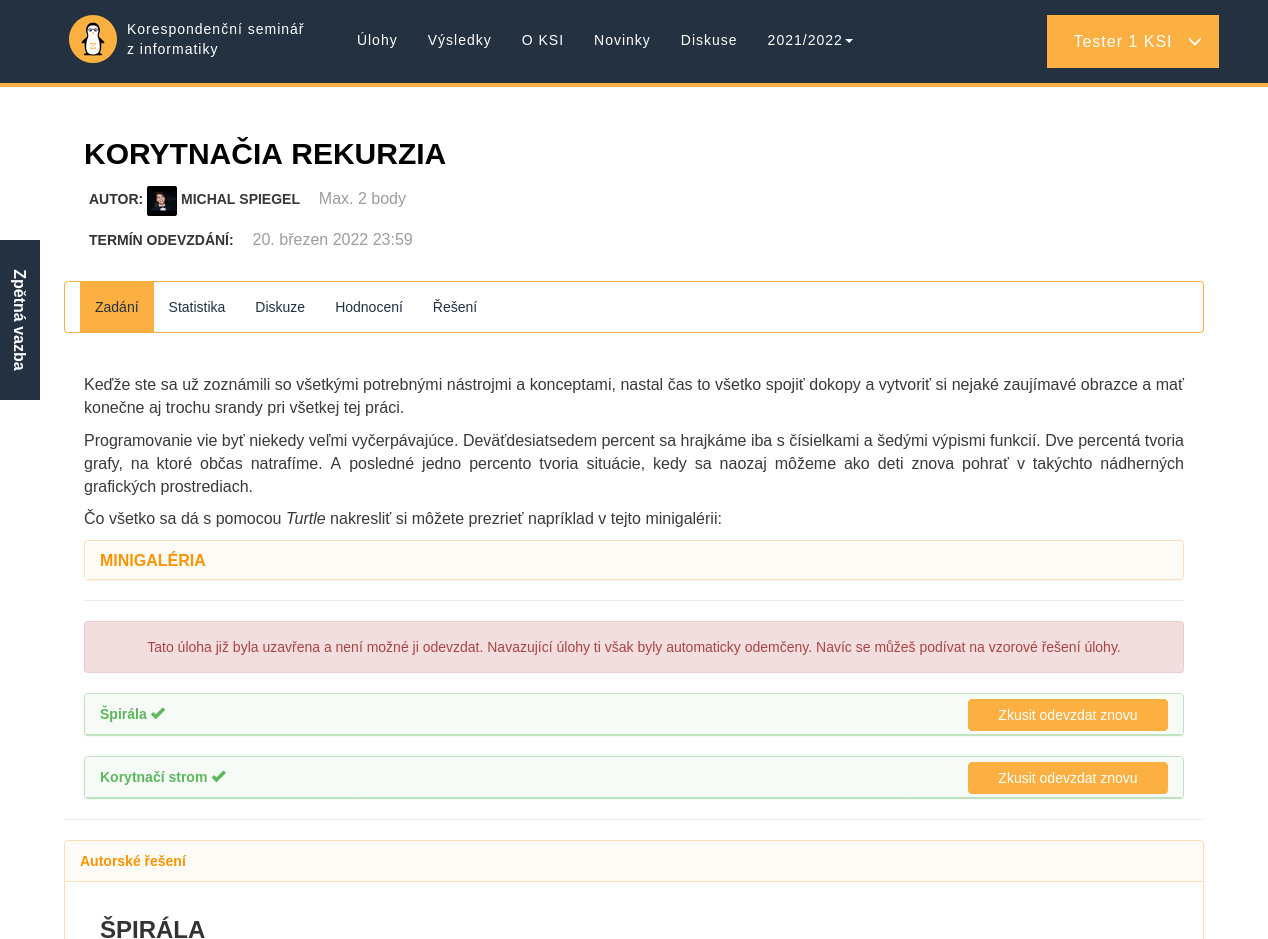
\includegraphics[width=.9\textwidth]{assets/img/task-curr}
\caption{The current look of a \acrshort{KSI} task}
\label{fig:task-curr}
\end{figure}

\begin{figure}
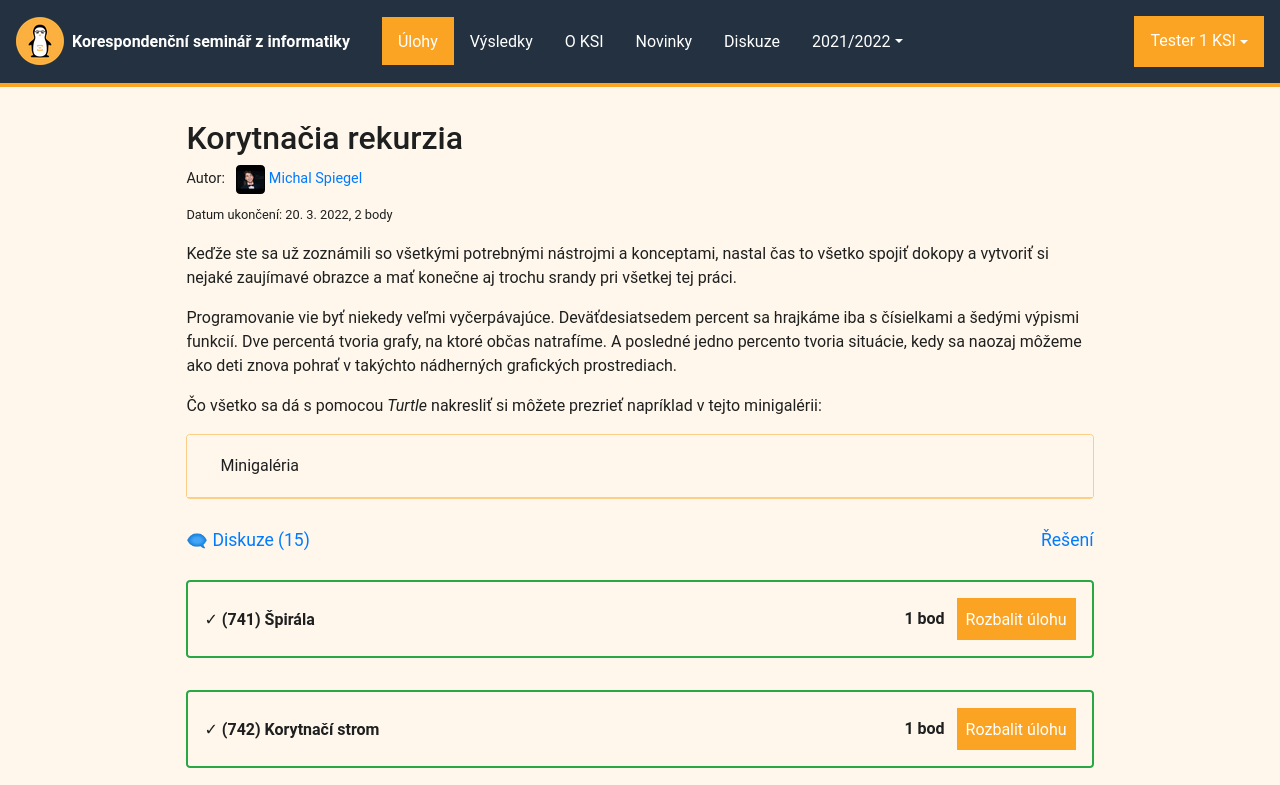
\includegraphics[width=\textwidth]{assets/img/task-new}
\caption{The new design of a \acrshort{KSI} task}
\label{fig:task-new}
\end{figure}


### Discussion page

The discussion forum on the \acrshort{KSI} web consists of two pages -- first, the selection of discussion subject thread and then posts within the tread.

#### Discussion selection

The selection takes the form of a table with the thread's name and its post count. The most notable difference between the current (\autoref{fig:discussroot-curr}) and new (\autoref{fig:discussroot-new}) design is that the current version contains a third column with a count of unread posts inside the thread. This column is always visible, even if all posts have been read. Moreover, it shows white text on an orange background, which may be difficult to read. In the new design, the count of the unread posts is shown only if there are any and is shown as a bold text in the post count column, making it easier for quick navigation.

\begin{figure}
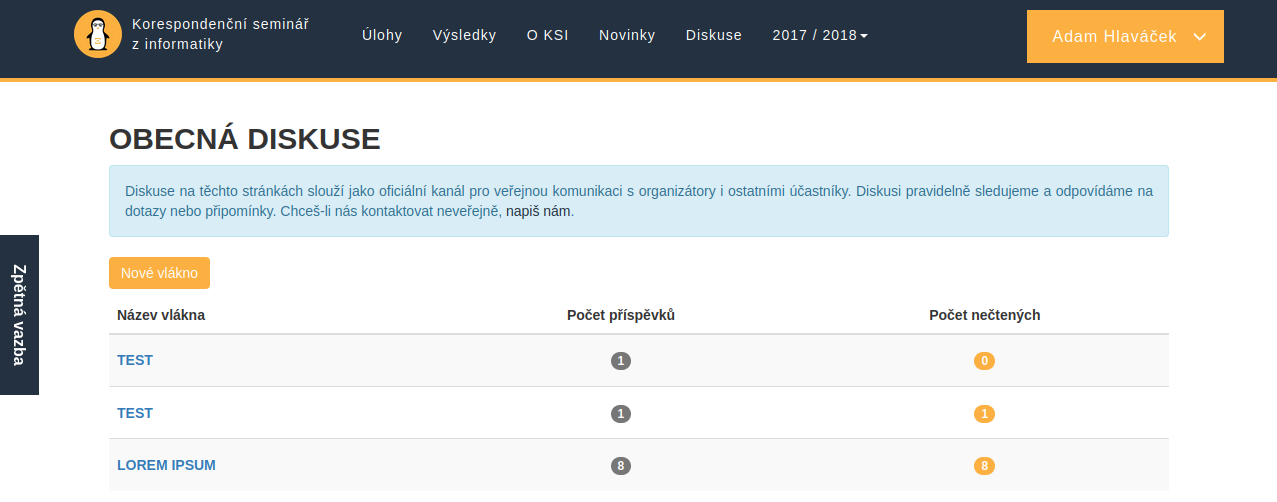
\includegraphics[width=\textwidth]{assets/img/discussionroot-curr}
\caption{The current look of a \acrshort{KSI} discussion selection page}
\label{fig:discussroot-curr}
\end{figure}

\begin{figure}
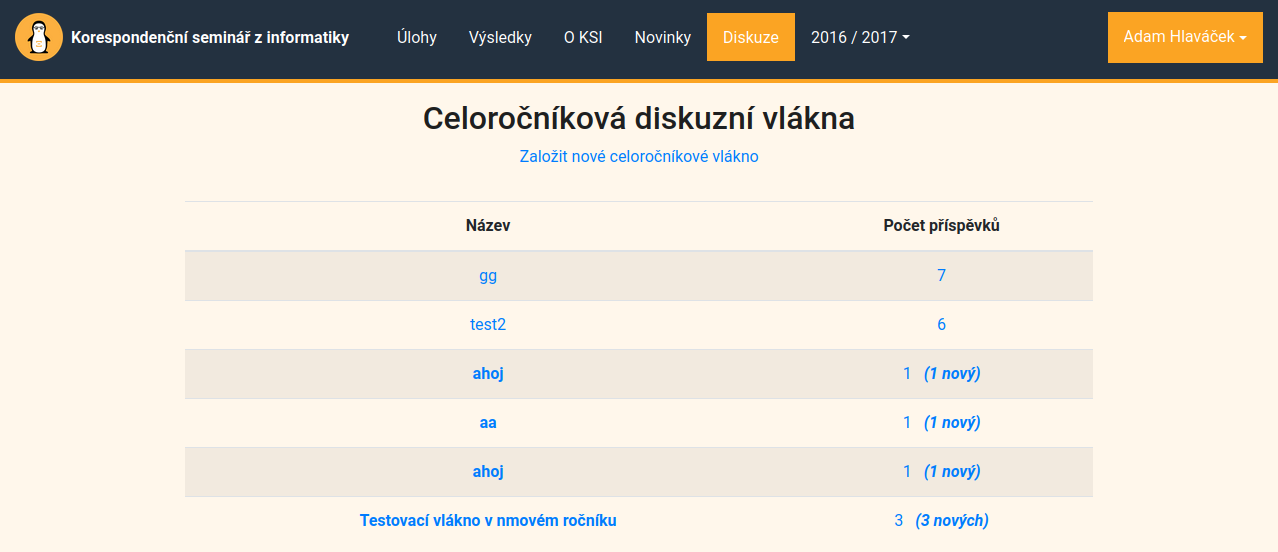
\includegraphics[width=\textwidth]{assets/img/discussionroot-new}
\caption{The new design of a \acrshort{KSI} discussion selection page}
\label{fig:discussroot-new}
\end{figure}

#### Discussion posts

In the current version (\autoref{fig:discuss-curr}), the posts have no borders and responses to a previous post is differentiated by a larger offset. However, if the posts receive multiple replies, it may overflow the maximum offset, which makes identifying which posts responds to which a difficult task. The new design of the web applications addresses these issues by adding borders to posts and rails that indicate which post is the parent of which reply. If the level of replies is too deep, then an additional button to unpack and continue within the reply thread is shown. When a reply thread is unpacked, it becomes the topmost post, hiding every post with a lesser level. By manually unpacking replies, the web application assures that the structure of posts will never overflow maximum offset and, as such, will always be easily readable. A newly added feature is a unique link to each post, making it easier to share it more precisely, rather than having to share the whole discussion thread and then manually search for the post content.

\begin{figure}
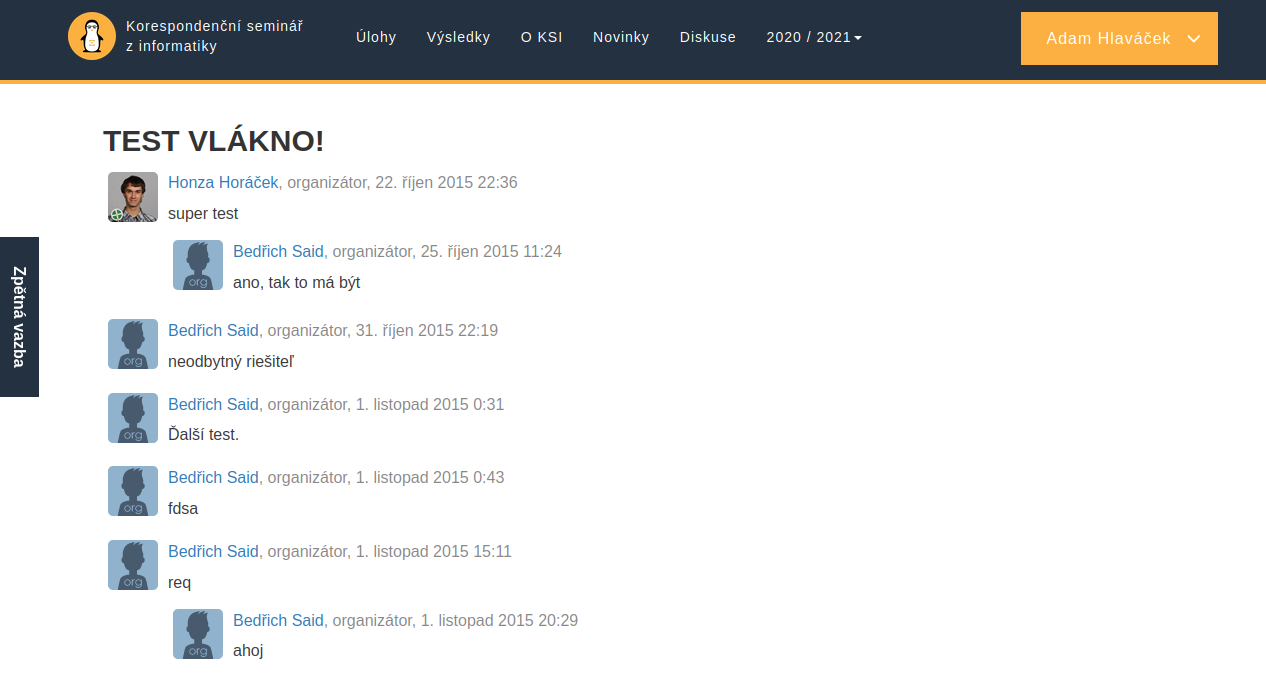
\includegraphics[width=\textwidth]{assets/img/discussion-curr}
\caption{The current look of a \acrshort{KSI} discussion posts}
\label{fig:discuss-curr}
\end{figure}

\begin{figure}
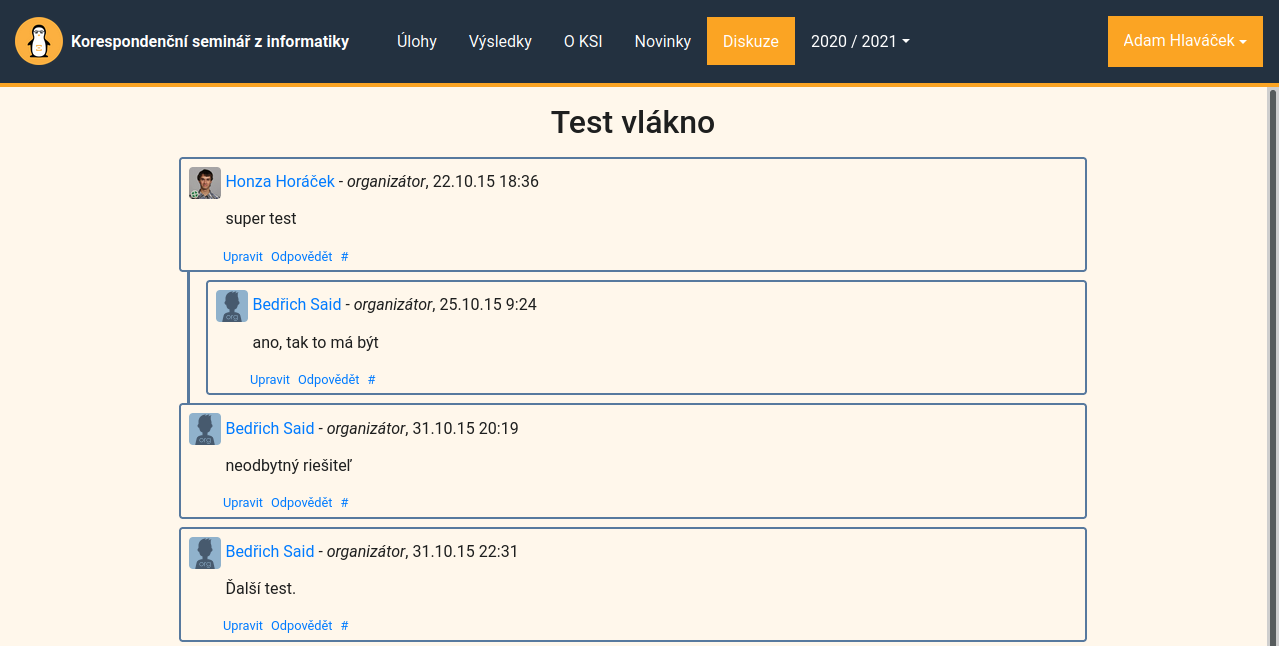
\includegraphics[width=\textwidth]{assets/img/discussion-new}
\caption{The new design of a \acrshort{KSI} discussion posts}
\label{fig:discuss-new}
\end{figure}

## The second instance

During the spring semester of 2022, the \acrshort{KSI} organizer team was contacted by a representative of the \acrshort{FI} \acrshort{MU} about creating a new online seminar for the newly accepted students with the same basic structure as \acrshort{KSI}. Participants will procedurally solve tasks about various subjects related to the informatics field and the university's environment in general. Because the new web application was developed with modularity in mind, it was selected as the main frontend for the new online seminar. The main adaptation tasks were changing the used colour pallet from \acrshort{KSI}'s to the one used by the official \acrshort{FI} \acrshort{MU} website and rewriting occurrences of \acrshort{KSI} to the name of the new seminar, together with renaming affected path names. Because all this information is kept in separate files, which are then referenced by the rest of the frontend, the process of modifying the values to the desired outcome is not time-consuming. Furthermore, the following updates applied to the parent project can be applied to the \fnurl{second instalment}{https://github.com/fi-naskoc/web-frontend-angular} by simply rebasing the patch commits on top of the new main branch of the parent project. The new online seminar, called \fnurl{Jump-start the \acrshort{FI}}{https://naskoc.fi.muni.cz/}, is set to begin at the end of May 2022.

\begin{figure}
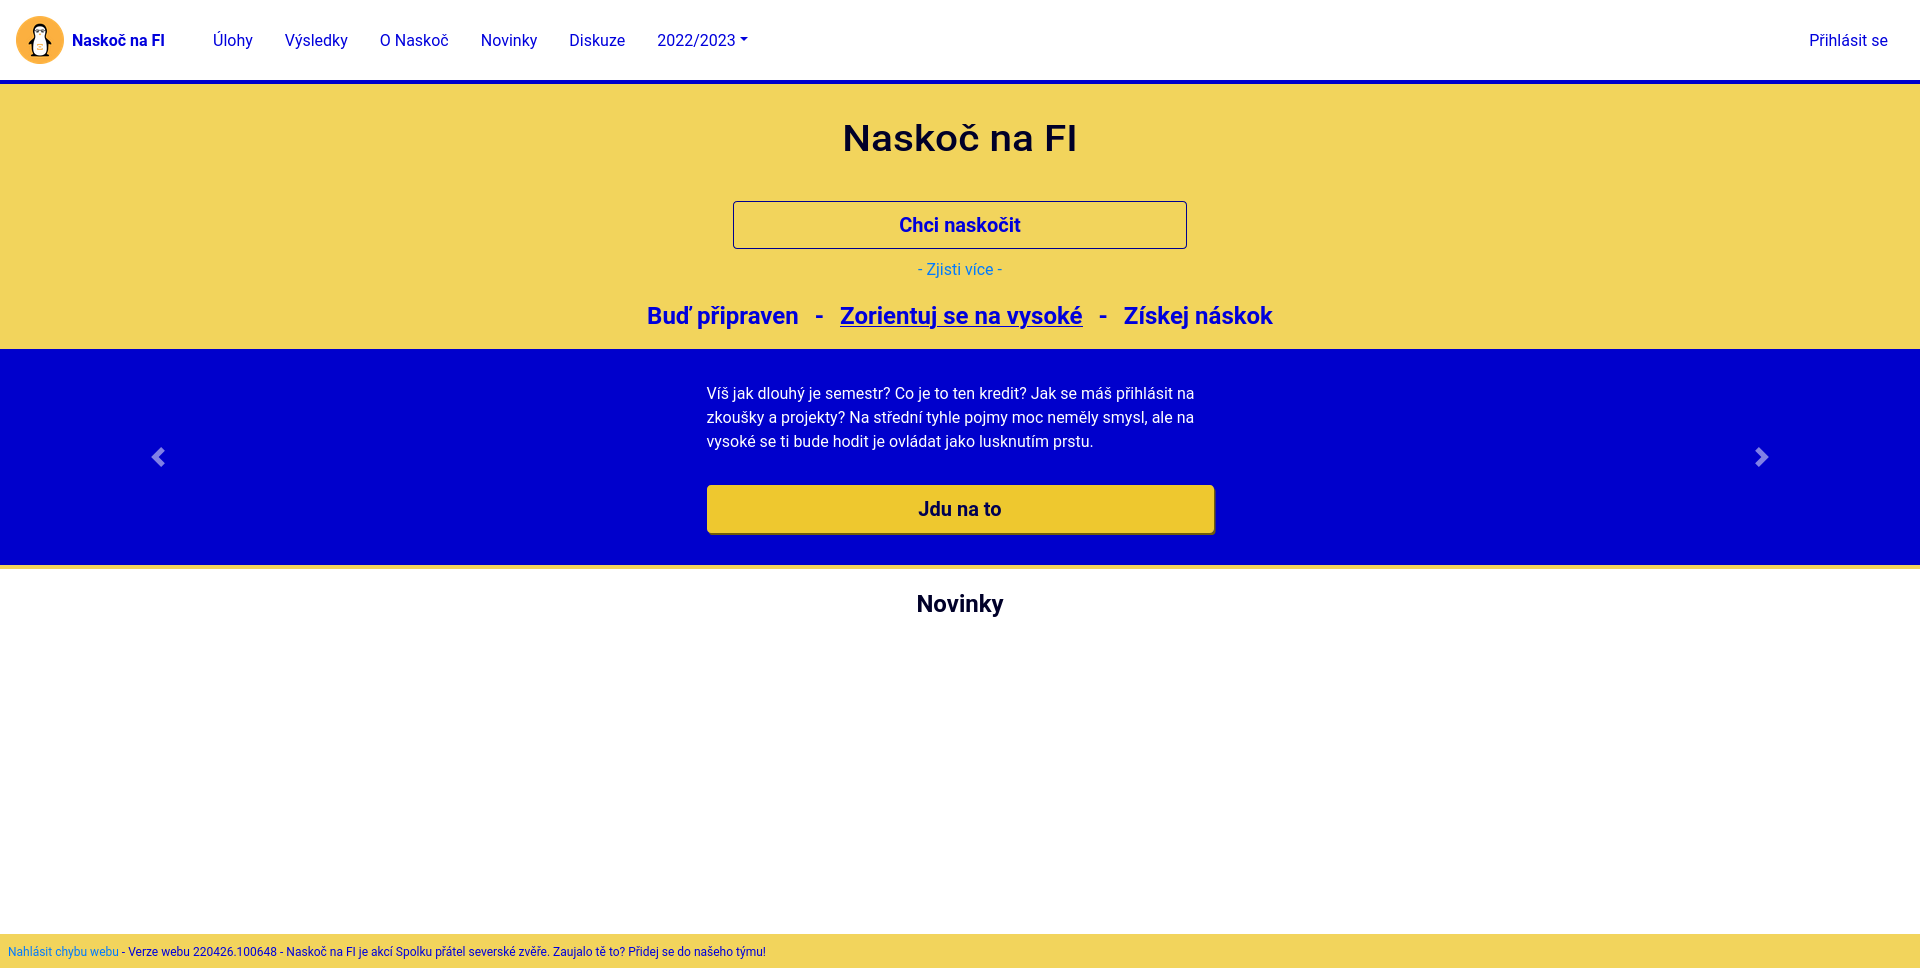
\includegraphics[width=\textwidth]{assets/img/naskoc-na-fi}
\caption{The welcome page for Jump-start the \acrshort{FI}}
\label{fig:naskoc-na-fi}
\end{figure}

## Restoring historic \acrshort{KSI} tasks

Before \acrshort{KSI} was transformed into an online competition, all assignments were sent to the participants through traditional mail. As such, the tasks were written as \LaTeX{} files, which were then built into a final \acrshort{PDF} for printing. This format is incompatible with current tasks written as markdown files and then converted to HTML on the backend. Still, these historic tasks have undeniable educational value, so making them easily accessible online	was set as one of the secondary goals of this thesis.

Because the backend converts internally the tasks written in markdown to HTML, it is possible to convert the \LaTeX{} to HTML directly with a tool \fnurl{`latex2html`}{https://www.latex2html.org/}, which can be later inserted into the database directly. Whenever `latex2html` encounters a part of a file that it cannot translate into HTML, it renders it as a \acrshort{PNG} or \acrshort{SVG} image and attaches it to the final HTML file. This operation is also performed on blocks with TeX mathematics and source code, both for which the \acrshort{KSI} web has direct support.

To improve the user's experience, as part of the postprocessing of the generated HTML, the original TeX math content is obtained from the alternative text of the respective image from HTML. Additionally, most \acrshort{SVG} images created by the tool contain a large transparent margin that must be removed. Finally, all images are embedded into the HTML code to contain all assets inside a single HTML file.

After all tasks are converted into their HTML variants, it is possible to generate a SQL script, which will insert the tasks into the database. The script divides the tasks by their year and wave while maintaining their relative order by using \acrshort{KSI} prerequisites. A module for submitting a solution with correct points will be shown if the source task was assigned a number of points.

Currently, the tasks are accessible only through the public development \acrshort{KSI} instance -- for example, the task \fnurl{"Atlas"}{https://ksi.ahlava.cz/ulohy/183} from the fifth wave of the 2009 year. Before deploying these historic tasks on the production server, a more extensive discussion with the \acrshort{KSI} organizers teams is needed, as follow up tasks, such as creating icons, may be required first. This discussion is planned for the summer of 2022. The source code of this converter is \fnurl{publicly available}{https://github.com/fi-ksi/seminar-till-2014-converter}.

## Evaluating the new web application

Since October 2021, the \acrshort{KSI} organizers were encouraged to submit their feedback on the state of the new web frontend. The new frontend was scheduled to be made public with a release of the last wave of the \acrshort{KSI} year 2021/2022. The organizers have submitted nine bug reports and ten feature suggestions through the designated form until that date. With the release of the last wave of the \acrshort{KSI} year 2021/2022, the feedback was also opened to the participants, together with a questionnaire for them to fill out. The participants were motivated to fill out the questionnaire by awarding a virtual trophy to everyone who submitted it.

### Questionnaire

The questionnaire sent to the \acrshort{KSI} participants consisted of three parts. In the first part, the participants were asked to provide their opinion on two new experimental \acrshort{UX} features (capitalization of the tasks title and design of a sortable module). The second section consisted of questions about comparing the new and current \acrshort{KSI} web frontend. As the answers, the participants were asked to choose a number between 1 and 5, where one is the best and five is the worst. The last section was made of free form questions about what participants think has improved with a new web and what was better on the current web frontend. A total of 21 participants have submitted the form.

#### Devices and responsiveness

Most participants who submitted the questionnaire have tested the new web on both desktop computers and mobile devices (81 \%, \autoref{fig:q-device}).

\begin{figure}
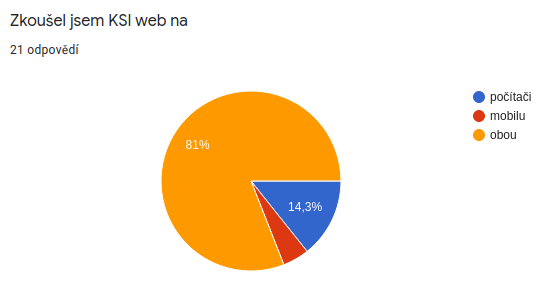
\includegraphics[width=.5\textwidth]{assets/img/questionare/device}
\caption{Questionnaire: Used devices devices}
\label{fig:q-device}
\end{figure}


#### Subjective speed

A total of 57.2 \% of respondents have answered that the new web application is faster than the current one, and 38.1 \% consider the responsiveness of both frontends to be on a similar level (\autoref{fig:q-speed}).

\begin{figure}
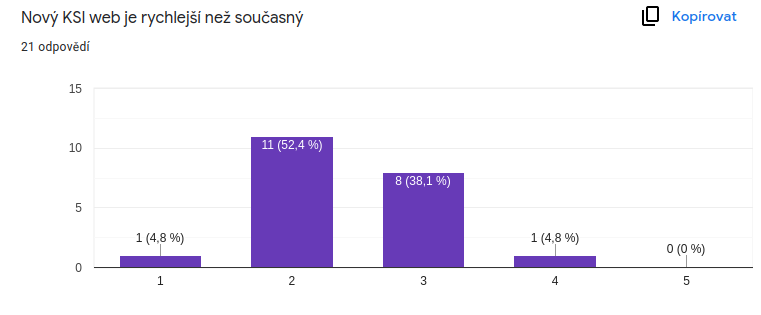
\includegraphics[width=\textwidth]{assets/img/questionare/faster}
\caption{Questionnaire: I find the new \acrshort{KSI} web faster than the current}
\label{fig:q-speed}
\end{figure}


#### User experience and user interface design

Even though most participants agree that the \acrshort{UX} and \acrshort{UI} on the desktop is better or the same (81 \%, \autoref{fig:q-ux-pc}; 95.2 \%, \autoref{fig:q-ui-pc}), the difference is most notable on the mobile phone. For the mobile version, the total of 90.5 \% for the \acrshort{UX} (\autoref{fig:q-ux-mobile}) and  85.7 \% for the \acrshort{UI} (\autoref{fig:q-ui-mobile}) thinks that the new web application is better than the current one.

\begin{figure}
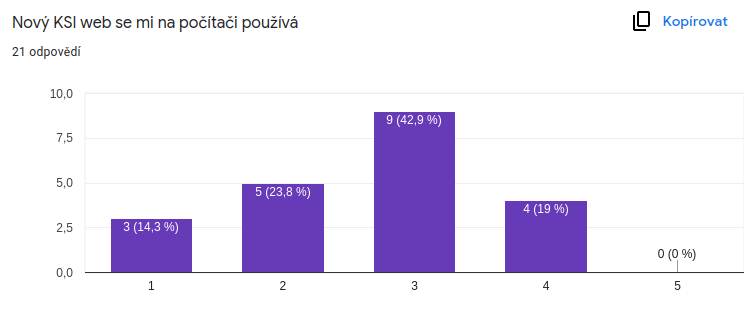
\includegraphics[width=\textwidth]{assets/img/questionare/pc-ux}
\caption{Questionnaire: My experience with the new \acrshort{KSI} web on desktop is better}
\label{fig:q-ux-pc}
\end{figure}

\begin{figure}
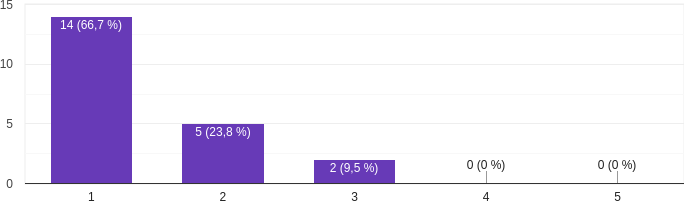
\includegraphics[width=\textwidth]{assets/img/questionare/mobile-ux}
\caption{Questionnaire: My experience with the new \acrshort{KSI} web on mobile is better}
\label{fig:q-ux-mobile}
\end{figure}

\begin{figure}
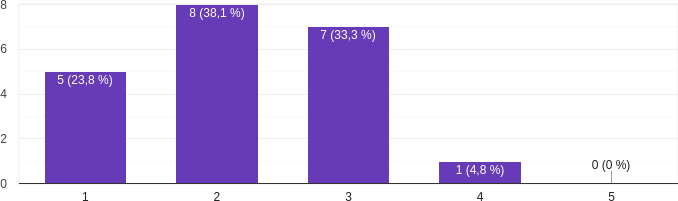
\includegraphics[width=\textwidth]{assets/img/questionare/pc-ui}
\caption{Questionnaire: The design of the new \acrshort{KSI} web interface on desktop is better}
\label{fig:q-ui-pc}
\end{figure}

\begin{figure}
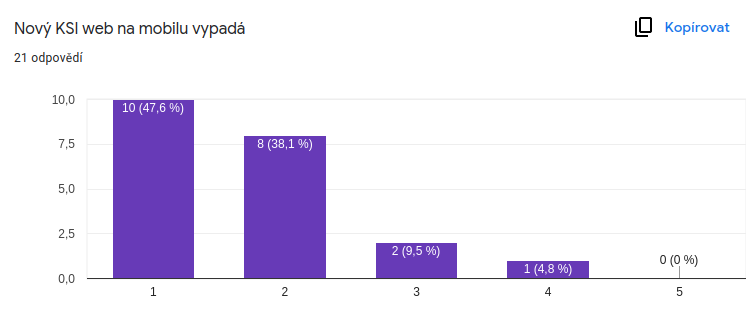
\includegraphics[width=\textwidth]{assets/img/questionare/mobile-ui}
\caption{Questionnaire: The design of the new \acrshort{KSI} web interface on mobile is better}
\label{fig:q-ui-mobile}
\end{figure}

# Conclusion

The primary goal of this thesis was to create a new web application for the Online Seminar of Informatics, together with eventual modifications to its backend. This goal was to be completed with a focus on long-term maintainability and easy modifiability. The secondary goals of this thesis were to make the new web application at least partially available on mobile devices, overall \acrshort{UX} improvements and republishing historic \acrshort{KSI} tasks which were previously incompatible with the current \acrshort{KSI} infrastructure.

First, I have analyzed from what components is the \acrshort{KSI} frontend made of and then described the current technological state of both the frontend and backend. Next, I have outlined the possible advantages and drawbacks of commonly used frameworks that were considered for the implementation part of this thesis regarding the capabilities of the \acrshort{KSI} organizers team for long-term support.

Before the development of the new web frontend, changes were made to the \acrshort{KSI} backend to ensure a more robust process that tries to minimize possible risks of miscommunication when passing requests between these two projects. After the backend changes were completed, I described specific changes and decisions behind the application architecture and user interface. The new application reuses only text and image assets and a colour palette.

Throughout the development process, the \acrshort{KSI} organizer team members submitted multiple enhancement ideas and discovered bugs, most of which were already incorporated into the project's code. The remaining discovered bugs require further discussion, as they may require performing breaking changes to the backend. To evaluate the final web application, a questionnaire about their experience with the application was sent to the \acrshort{KSI} participants. The responses to the questionnaire were positive, most notably in relation to the mobile version of the web application, which is now entirely usable with all features available from the desktop version.

At the final meeting of the \acrshort{KSI}, organizers teams decided that the new web application will replace the current one with the start of the \acrshort{KSI} year 2022/2023 in September. In the meantime, the new web application is already being used in a new online activity from the Faculty of Informatics at Masaryk University, which is set to launch on the 25th of May 2022. For this new activity, the web application's colour schema and internationalization texts were modified to meet the activity's requirements. No more significant changes were required, underlining the goal of easy modifiability.

In the future, the new web application is expected to be further actively developed. This subsequent development will reflect breaking changes that are to be made to the \acrshort{KSI} backend, which will make the current web frontend unusable and is scheduled for the summer of 2022. These changes could not be performed before because breaking changes were deemed unsafe while the \acrshort{KSI} year was in progress. Furthermore, the historic \acrshort{KSI} tasks, which are now available on the public \acrshort{KSI} testing server, are to be merged with the production database after additional steps like creating icons to better fit in with the rest of the tasks. All these tasks also require a heavy cooperation of multiple people, which is why it was scheduled outside the university semester.

Because all projects created as part of this thesis are published under \fnurl{GNU General Public License v3.0}{https://choosealicense.com/licenses/gpl-3.0/}, they may be freely used by anyone.

\end{markdown*}

\shorthandon{-}
  \printbibliography[heading=bibintoc] %% Print the bibliography.

  \makeatletter\thesis@blocks@clear\makeatother
%  \phantomsection %% Print the index and insert it into the
%  \addcontentsline{toc}{chapter}{\indexname} %% table of contents.
%  \printindex

\appendix %% Start the appendices.
\chapter{An appendix}

\mdstart

The implementation of this thesis is submitted to the archive as a `.tar.gz` archive, which contains all three projects as root folders -- the web application frontend, the Swagger backend proxy project and the project for the conversion of \LaTeX{} tasks to the SQL statement. The archive, and every contained project's directory, contains a `README.md` file, which describes the structure and requirements for starting the project.

\end{markdown*}

\end{document}
